\documentclass[twoside]{book}

% Packages required by doxygen
\usepackage{fixltx2e}
\usepackage{calc}
\usepackage{doxygen}
\usepackage[export]{adjustbox} % also loads graphicx
\usepackage{graphicx}
\usepackage[utf8]{inputenc}
\usepackage{makeidx}
\usepackage{multicol}
\usepackage{multirow}
\PassOptionsToPackage{warn}{textcomp}
\usepackage{textcomp}
\usepackage[nointegrals]{wasysym}
\usepackage[table]{xcolor}

% Font selection
\usepackage[T1]{fontenc}
\usepackage[scaled=.90]{helvet}
\usepackage{courier}
\usepackage{amssymb}
\usepackage{sectsty}
\renewcommand{\familydefault}{\sfdefault}
\allsectionsfont{%
  \fontseries{bc}\selectfont%
  \color{darkgray}%
}
\renewcommand{\DoxyLabelFont}{%
  \fontseries{bc}\selectfont%
  \color{darkgray}%
}
\newcommand{\+}{\discretionary{\mbox{\scriptsize$\hookleftarrow$}}{}{}}

% Page & text layout
\usepackage{geometry}
\geometry{%
  a4paper,%
  top=2.5cm,%
  bottom=2.5cm,%
  left=2.5cm,%
  right=2.5cm%
}
\tolerance=750
\hfuzz=15pt
\hbadness=750
\setlength{\emergencystretch}{15pt}
\setlength{\parindent}{0cm}
\setlength{\parskip}{0.2cm}
\makeatletter
\renewcommand{\paragraph}{%
  \@startsection{paragraph}{4}{0ex}{-1.0ex}{1.0ex}{%
    \normalfont\normalsize\bfseries\SS@parafont%
  }%
}
\renewcommand{\subparagraph}{%
  \@startsection{subparagraph}{5}{0ex}{-1.0ex}{1.0ex}{%
    \normalfont\normalsize\bfseries\SS@subparafont%
  }%
}
\makeatother

% Headers & footers
\usepackage{fancyhdr}
\pagestyle{fancyplain}
\fancyhead[LE]{\fancyplain{}{\bfseries\thepage}}
\fancyhead[CE]{\fancyplain{}{}}
\fancyhead[RE]{\fancyplain{}{\bfseries\leftmark}}
\fancyhead[LO]{\fancyplain{}{\bfseries\rightmark}}
\fancyhead[CO]{\fancyplain{}{}}
\fancyhead[RO]{\fancyplain{}{\bfseries\thepage}}
\fancyfoot[LE]{\fancyplain{}{}}
\fancyfoot[CE]{\fancyplain{}{}}
\fancyfoot[RE]{\fancyplain{}{\bfseries\scriptsize Generated on Sun Nov 8 2015 21\+:15\+:52 for O\+L\+Z by Doxygen }}
\fancyfoot[LO]{\fancyplain{}{\bfseries\scriptsize Generated on Sun Nov 8 2015 21\+:15\+:52 for O\+L\+Z by Doxygen }}
\fancyfoot[CO]{\fancyplain{}{}}
\fancyfoot[RO]{\fancyplain{}{}}
\renewcommand{\footrulewidth}{0.4pt}
\renewcommand{\chaptermark}[1]{%
  \markboth{#1}{}%
}
\renewcommand{\sectionmark}[1]{%
  \markright{\thesection\ #1}%
}

% Indices & bibliography
\usepackage{natbib}
\usepackage[titles]{tocloft}
\setcounter{tocdepth}{3}
\setcounter{secnumdepth}{5}
\makeindex

% Hyperlinks (required, but should be loaded last)
\usepackage{ifpdf}
\ifpdf
  \usepackage[pdftex,pagebackref=true]{hyperref}
\else
  \usepackage[ps2pdf,pagebackref=true]{hyperref}
\fi
\hypersetup{%
  colorlinks=true,%
  linkcolor=blue,%
  citecolor=blue,%
  unicode%
}

% Custom commands
\newcommand{\clearemptydoublepage}{%
  \newpage{\pagestyle{empty}\cleardoublepage}%
}


%===== C O N T E N T S =====

\begin{document}

% Titlepage & ToC
\hypersetup{pageanchor=false,
             bookmarks=true,
             bookmarksnumbered=true,
             pdfencoding=unicode
            }
\pagenumbering{roman}
\begin{titlepage}
\vspace*{7cm}
\begin{center}%
{\Large O\+L\+Z }\\
\vspace*{1cm}
{\large Generated by Doxygen 1.8.10}\\
\vspace*{0.5cm}
{\small Sun Nov 8 2015 21:15:52}\\
\end{center}
\end{titlepage}
\clearemptydoublepage
\tableofcontents
\clearemptydoublepage
\pagenumbering{arabic}
\hypersetup{pageanchor=true}

%--- Begin generated contents ---
\chapter{Hierarchical Index}
\section{Class Hierarchy}
This inheritance list is sorted roughly, but not completely, alphabetically\+:\begin{DoxyCompactList}
\item \contentsline{section}{Advertisement}{\pageref{class_advertisement}}{}
\begin{DoxyCompactList}
\item \contentsline{section}{Purchase}{\pageref{class_purchase}}{}
\item \contentsline{section}{Sale}{\pageref{class_sale}}{}
\end{DoxyCompactList}
\item \contentsline{section}{Data}{\pageref{class_data}}{}
\item \contentsline{section}{Date}{\pageref{class_date}}{}
\item \contentsline{section}{Location}{\pageref{class_location}}{}
\item \contentsline{section}{Menu}{\pageref{class_menu}}{}
\begin{DoxyCompactList}
\item \contentsline{section}{Ad\+Display\+Menu}{\pageref{class_ad_display_menu}}{}
\item \contentsline{section}{Option\+Menu}{\pageref{class_option_menu}}{}
\item \contentsline{section}{Search\+Menu}{\pageref{class_search_menu}}{}
\end{DoxyCompactList}
\item \contentsline{section}{User}{\pageref{class_user}}{}
\end{DoxyCompactList}

\chapter{Class Index}
\section{Class List}
Here are the classes, structs, unions and interfaces with brief descriptions\+:\begin{DoxyCompactList}
\item\contentsline{section}{\hyperlink{class_ad_display_menu}{Ad\+Display\+Menu} \\*Code for class \hyperlink{class_ad_display_menu}{Ad\+Display\+Menu} }{\pageref{class_ad_display_menu}}{}
\item\contentsline{section}{\hyperlink{class_advertisement}{Advertisement} \\*\hyperlink{class_advertisement}{Advertisement} class }{\pageref{class_advertisement}}{}
\item\contentsline{section}{\hyperlink{class_data}{Data} \\*\hyperlink{class_user}{User} and \hyperlink{class_advertisement}{Advertisement} data class }{\pageref{class_data}}{}
\item\contentsline{section}{\hyperlink{class_date}{Date} \\*\hyperlink{class_date}{Date} class }{\pageref{class_date}}{}
\item\contentsline{section}{\hyperlink{class_location}{Location} \\*Code for class \hyperlink{class_location}{Location}. A county has many cities; a district has various counties }{\pageref{class_location}}{}
\item\contentsline{section}{\hyperlink{class_menu}{Menu} \\*\hyperlink{class_menu}{Menu} class }{\pageref{class_menu}}{}
\item\contentsline{section}{\hyperlink{class_option_menu}{Option\+Menu} \\*\hyperlink{class_option_menu}{Option\+Menu} class }{\pageref{class_option_menu}}{}
\item\contentsline{section}{\hyperlink{class_purchase}{Purchase} \\*\hyperlink{class_purchase}{Purchase} class }{\pageref{class_purchase}}{}
\item\contentsline{section}{\hyperlink{class_sale}{Sale} \\*\hyperlink{class_sale}{Sale} class }{\pageref{class_sale}}{}
\item\contentsline{section}{\hyperlink{class_search_menu}{Search\+Menu} \\*\hyperlink{class_search_menu}{Search\+Menu} class }{\pageref{class_search_menu}}{}
\item\contentsline{section}{\hyperlink{class_user}{User} \\*\hyperlink{class_user}{User} class }{\pageref{class_user}}{}
\end{DoxyCompactList}

\chapter{File Index}
\section{File List}
Here is a list of all documented files with brief descriptions\+:\begin{DoxyCompactList}
\item\contentsline{section}{O\+L\+Z/src/{\bfseries enums.\+h} }{\pageref{enums_8h}}{}
\item\contentsline{section}{O\+L\+Z/src/class/advertisement/\hyperlink{advertisement_8cpp}{advertisement.\+cpp} \\*Code for class \hyperlink{class_advertisement}{Advertisement} }{\pageref{advertisement_8cpp}}{}
\item\contentsline{section}{O\+L\+Z/src/class/advertisement/\hyperlink{advertisement_8h}{advertisement.\+h} \\*Header file for class \hyperlink{class_advertisement}{Advertisement} }{\pageref{advertisement_8h}}{}
\item\contentsline{section}{O\+L\+Z/src/class/advertisement/purchase/\hyperlink{purchase_8cpp}{purchase.\+cpp} \\*Code for class \hyperlink{class_purchase}{Purchase} }{\pageref{purchase_8cpp}}{}
\item\contentsline{section}{O\+L\+Z/src/class/advertisement/purchase/\hyperlink{purchase_8h}{purchase.\+h} \\*Header file for class \hyperlink{class_purchase}{Purchase} }{\pageref{purchase_8h}}{}
\item\contentsline{section}{O\+L\+Z/src/class/advertisement/sale/\hyperlink{sale_8cpp}{sale.\+cpp} \\*Code for class \hyperlink{class_sale}{Sale} }{\pageref{sale_8cpp}}{}
\item\contentsline{section}{O\+L\+Z/src/class/advertisement/sale/\hyperlink{sale_8h}{sale.\+h} \\*Header file for class \hyperlink{class_sale}{Sale} }{\pageref{sale_8h}}{}
\item\contentsline{section}{O\+L\+Z/src/class/data/{\bfseries data.\+h} }{\pageref{data_8h}}{}
\item\contentsline{section}{O\+L\+Z/src/class/date/{\bfseries date.\+h} }{\pageref{date_8h}}{}
\item\contentsline{section}{O\+L\+Z/src/class/location/{\bfseries location.\+h} }{\pageref{location_8h}}{}
\item\contentsline{section}{O\+L\+Z/src/class/menu/{\bfseries menu.\+h} }{\pageref{menu_8h}}{}
\item\contentsline{section}{O\+L\+Z/src/class/menu/ad\+Display\+Menu/{\bfseries ad\+Display\+Menu.\+h} }{\pageref{ad_display_menu_8h}}{}
\item\contentsline{section}{O\+L\+Z/src/class/menu/option\+Menu/{\bfseries option\+Menu.\+h} }{\pageref{option_menu_8h}}{}
\item\contentsline{section}{O\+L\+Z/src/class/menu/search\+Menu/{\bfseries search\+Menu.\+h} }{\pageref{search_menu_8h}}{}
\item\contentsline{section}{O\+L\+Z/src/class/user/{\bfseries user.\+h} }{\pageref{user_8h}}{}
\item\contentsline{section}{O\+L\+Z/src/menus/main\+Menu/{\bfseries main\+Menu.\+h} }{\pageref{main_menu_8h}}{}
\end{DoxyCompactList}

\chapter{Class Documentation}
\hypertarget{class_ad_display_menu}{}\section{Ad\+Display\+Menu Class Reference}
\label{class_ad_display_menu}\index{Ad\+Display\+Menu@{Ad\+Display\+Menu}}


Code for class \hyperlink{class_ad_display_menu}{Ad\+Display\+Menu}.  




{\ttfamily \#include $<$ad\+Display\+Menu.\+h$>$}

Inheritance diagram for Ad\+Display\+Menu\+:\begin{figure}[H]
\begin{center}
\leavevmode
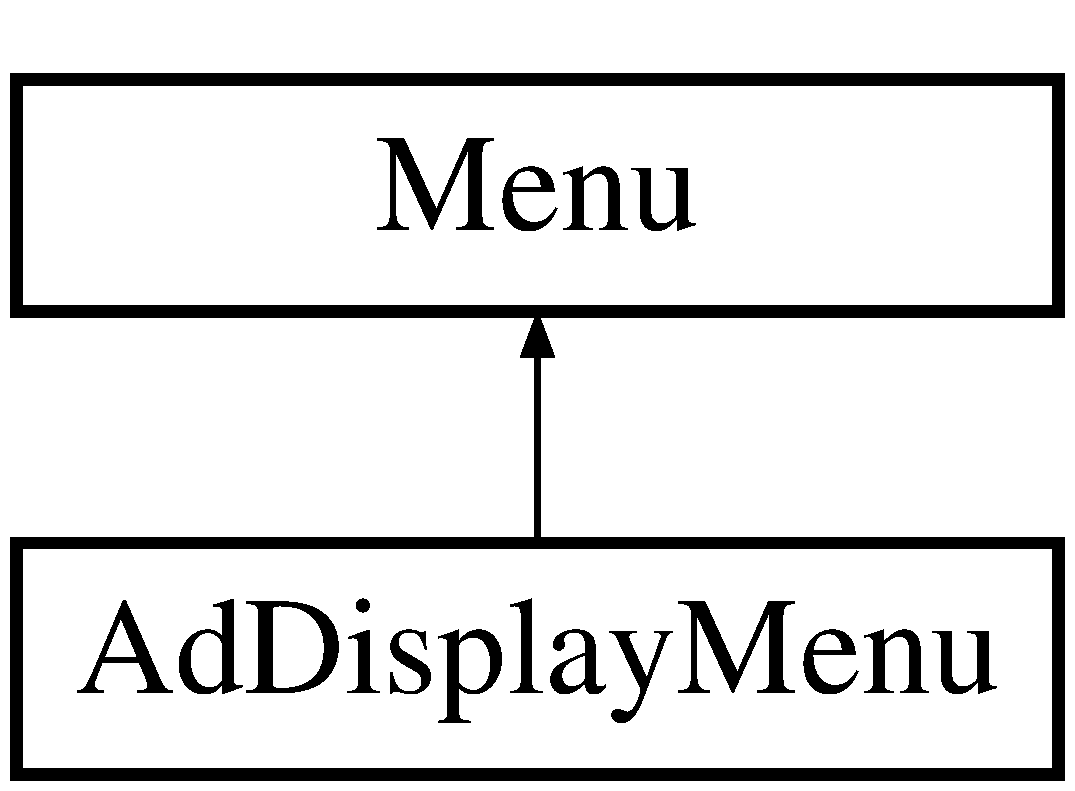
\includegraphics[height=2.000000cm]{class_ad_display_menu}
\end{center}
\end{figure}
\subsection*{Public Member Functions}
\begin{DoxyCompactItemize}
\item 
\hyperlink{class_ad_display_menu_a0b3787752d998c2c0fbb38b0086c4b15}{Ad\+Display\+Menu} (\hyperlink{class_data}{Data} $\ast$data, \hyperlink{class_advertisement}{Advertisement} $\ast$ad, unsigned int height=20, unsigned int width=50, char border\+Char= \textquotesingle{}\#\textquotesingle{})
\begin{DoxyCompactList}\small\item\em Constructor for \hyperlink{class_ad_display_menu}{Ad\+Display\+Menu} class. \end{DoxyCompactList}\item 
\hypertarget{class_ad_display_menu_acf175cade9d9e5a6d65f1eb901f17a84}{}void \hyperlink{class_ad_display_menu_acf175cade9d9e5a6d65f1eb901f17a84}{print} ()\label{class_ad_display_menu_acf175cade9d9e5a6d65f1eb901f17a84}

\begin{DoxyCompactList}\small\item\em Prints the menu to the screen. \end{DoxyCompactList}\item 
\hypertarget{class_ad_display_menu_ae10113101504905c1cf802085c603a8b}{}void \hyperlink{class_ad_display_menu_ae10113101504905c1cf802085c603a8b}{create\+Menu} ()\label{class_ad_display_menu_ae10113101504905c1cf802085c603a8b}

\begin{DoxyCompactList}\small\item\em Calls print and creates the interaction with the user. \end{DoxyCompactList}\end{DoxyCompactItemize}
\subsection*{Additional Inherited Members}


\subsection{Detailed Description}
Code for class \hyperlink{class_ad_display_menu}{Ad\+Display\+Menu}. 

\subsection{Constructor \& Destructor Documentation}
\hypertarget{class_ad_display_menu_a0b3787752d998c2c0fbb38b0086c4b15}{}\index{Ad\+Display\+Menu@{Ad\+Display\+Menu}!Ad\+Display\+Menu@{Ad\+Display\+Menu}}
\index{Ad\+Display\+Menu@{Ad\+Display\+Menu}!Ad\+Display\+Menu@{Ad\+Display\+Menu}}
\subsubsection[{Ad\+Display\+Menu(\+Data $\ast$data, Advertisement $\ast$ad, unsigned int height=20, unsigned int width=50, char border\+Char= \textquotesingle{}\#\textquotesingle{})}]{\setlength{\rightskip}{0pt plus 5cm}Ad\+Display\+Menu\+::\+Ad\+Display\+Menu (
\begin{DoxyParamCaption}
\item[{{\bf Data} $\ast$}]{data, }
\item[{{\bf Advertisement} $\ast$}]{ad, }
\item[{unsigned int}]{height = {\ttfamily 20}, }
\item[{unsigned int}]{width = {\ttfamily 50}, }
\item[{char}]{border\+Char = {\ttfamily \textquotesingle{}\#\textquotesingle{}}}
\end{DoxyParamCaption}
)}\label{class_ad_display_menu_a0b3787752d998c2c0fbb38b0086c4b15}


Constructor for \hyperlink{class_ad_display_menu}{Ad\+Display\+Menu} class. 


\begin{DoxyParams}{Parameters}
{\em \hyperlink{class_data}{Data}} & data \\
\hline
{\em ad} & \hyperlink{class_advertisement}{Advertisement} to display \\
\hline
{\em height} & \hyperlink{class_menu}{Menu} height \\
\hline
{\em width} & \hyperlink{class_menu}{Menu} width \\
\hline
{\em border\+Char} & Character with which to fill the menu borders \\
\hline
\end{DoxyParams}


The documentation for this class was generated from the following files\+:\begin{DoxyCompactItemize}
\item 
O\+L\+Z/src/class/menu/ad\+Display\+Menu/\hyperlink{ad_display_menu_8h}{ad\+Display\+Menu.\+h}\item 
O\+L\+Z/src/class/menu/ad\+Display\+Menu/\hyperlink{ad_display_menu_8cpp}{ad\+Display\+Menu.\+cpp}\end{DoxyCompactItemize}

\hypertarget{class_advertisement}{}\section{Advertisement Class Reference}
\label{class_advertisement}\index{Advertisement@{Advertisement}}


\hyperlink{class_advertisement}{Advertisement} class.  




{\ttfamily \#include $<$advertisement.\+h$>$}

Inheritance diagram for Advertisement\+:\begin{figure}[H]
\begin{center}
\leavevmode
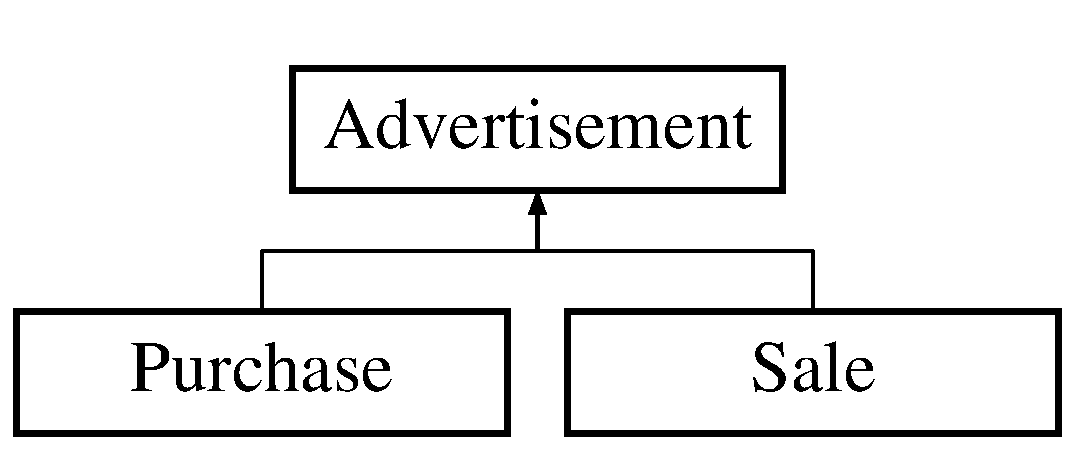
\includegraphics[height=2.000000cm]{class_advertisement}
\end{center}
\end{figure}
\subsection*{Public Member Functions}
\begin{DoxyCompactItemize}
\item 
\hyperlink{class_advertisement_a3819a25a48afbca0a6da6717ef0d6da3}{Advertisement} (\hyperlink{class_user}{User} $\ast$owner, string title, Category category)
\begin{DoxyCompactList}\small\item\em Constructor for class \hyperlink{class_advertisement}{Advertisement}. \end{DoxyCompactList}\item 
\hyperlink{class_advertisement_a343d31bb9f21892718fc4a756f7eb05c}{Advertisement} (\hyperlink{class_user}{User} $\ast$owner, string title, Category category, string description)
\begin{DoxyCompactList}\small\item\em Constructor for class \hyperlink{class_advertisement}{Advertisement}. \end{DoxyCompactList}\item 
\hypertarget{class_advertisement_a49170a22dcd2a8bf88d3ed1aad475b82}{}virtual \hyperlink{class_advertisement_a49170a22dcd2a8bf88d3ed1aad475b82}{$\sim$\+Advertisement} ()\label{class_advertisement_a49170a22dcd2a8bf88d3ed1aad475b82}

\begin{DoxyCompactList}\small\item\em \hyperlink{class_advertisement}{Advertisement} destructor. \end{DoxyCompactList}\item 
unsigned int \hyperlink{class_advertisement_aa66d9158d12ae99a04f81cf2adb155fd}{get\+Id} () const 
\begin{DoxyCompactList}\small\item\em Gets advertisement I\+D. \end{DoxyCompactList}\item 
string \hyperlink{class_advertisement_ac65aa68caf2b1697c0cc04f2ebb0fd99}{get\+Title} () const 
\begin{DoxyCompactList}\small\item\em Gets advertisement title. \end{DoxyCompactList}\item 
Category \hyperlink{class_advertisement_a123c05d427fed1ac7fec0f55050da20d}{get\+Category} () const 
\begin{DoxyCompactList}\small\item\em Gets advertisement category. \end{DoxyCompactList}\item 
string \hyperlink{class_advertisement_ac455b4918dbd923af81efbaebf924985}{get\+Description} () const 
\begin{DoxyCompactList}\small\item\em Gets advertisement description. \end{DoxyCompactList}\item 
\hypertarget{class_advertisement_a260fbb1a64495a5e99591202389744a0}{}string {\bfseries get\+Image\+At} (unsigned int index) const \label{class_advertisement_a260fbb1a64495a5e99591202389744a0}

\item 
\hypertarget{class_advertisement_a3925f5b2411ae7ac00a56f3398ae9353}{}void {\bfseries add\+Image} (string path)\label{class_advertisement_a3925f5b2411ae7ac00a56f3398ae9353}

\item 
\hypertarget{class_advertisement_abd20373813b956bac9a6fd78a4947ebc}{}void \hyperlink{class_advertisement_abd20373813b956bac9a6fd78a4947ebc}{increment\+Views} ()\label{class_advertisement_abd20373813b956bac9a6fd78a4947ebc}

\begin{DoxyCompactList}\small\item\em Increments advertisement views. \end{DoxyCompactList}\item 
bool \hyperlink{class_advertisement_a883fc4cf6525ed95001f5c21c8a4d2ff}{search\+For\+Text} (string text) const 
\begin{DoxyCompactList}\small\item\em Searches for text in advertisement. \end{DoxyCompactList}\item 
virtual void \hyperlink{class_advertisement_acc122690eedc8eb9bfe1689d7d58052c}{display\+Ad} (unsigned int height, unsigned int width, char border\+Char)=0
\begin{DoxyCompactList}\small\item\em Displays ad. \end{DoxyCompactList}\end{DoxyCompactItemize}


\subsection{Detailed Description}
\hyperlink{class_advertisement}{Advertisement} class. 

\subsection{Constructor \& Destructor Documentation}
\hypertarget{class_advertisement_a3819a25a48afbca0a6da6717ef0d6da3}{}\index{Advertisement@{Advertisement}!Advertisement@{Advertisement}}
\index{Advertisement@{Advertisement}!Advertisement@{Advertisement}}
\subsubsection[{Advertisement(\+User $\ast$owner, string title, Category category)}]{\setlength{\rightskip}{0pt plus 5cm}Advertisement\+::\+Advertisement (
\begin{DoxyParamCaption}
\item[{{\bf User} $\ast$}]{owner, }
\item[{string}]{title, }
\item[{Category}]{category}
\end{DoxyParamCaption}
)}\label{class_advertisement_a3819a25a48afbca0a6da6717ef0d6da3}


Constructor for class \hyperlink{class_advertisement}{Advertisement}. 


\begin{DoxyParams}{Parameters}
{\em owner} & Pointer to advertisement owner \\
\hline
{\em title} & \hyperlink{class_advertisement}{Advertisement} title \\
\hline
{\em category} & \hyperlink{class_advertisement}{Advertisement} category \\
\hline
\end{DoxyParams}
\hypertarget{class_advertisement_a343d31bb9f21892718fc4a756f7eb05c}{}\index{Advertisement@{Advertisement}!Advertisement@{Advertisement}}
\index{Advertisement@{Advertisement}!Advertisement@{Advertisement}}
\subsubsection[{Advertisement(\+User $\ast$owner, string title, Category category, string description)}]{\setlength{\rightskip}{0pt plus 5cm}Advertisement\+::\+Advertisement (
\begin{DoxyParamCaption}
\item[{{\bf User} $\ast$}]{owner, }
\item[{string}]{title, }
\item[{Category}]{category, }
\item[{string}]{description}
\end{DoxyParamCaption}
)}\label{class_advertisement_a343d31bb9f21892718fc4a756f7eb05c}


Constructor for class \hyperlink{class_advertisement}{Advertisement}. 


\begin{DoxyParams}{Parameters}
{\em owner} & Pointer to advertisement owner \\
\hline
{\em title} & \hyperlink{class_advertisement}{Advertisement} title \\
\hline
{\em category} & \hyperlink{class_advertisement}{Advertisement} category \\
\hline
{\em description} & \hyperlink{class_advertisement}{Advertisement} description \\
\hline
\end{DoxyParams}


\subsection{Member Function Documentation}
\hypertarget{class_advertisement_acc122690eedc8eb9bfe1689d7d58052c}{}\index{Advertisement@{Advertisement}!display\+Ad@{display\+Ad}}
\index{display\+Ad@{display\+Ad}!Advertisement@{Advertisement}}
\subsubsection[{display\+Ad(unsigned int height, unsigned int width, char border\+Char)=0}]{\setlength{\rightskip}{0pt plus 5cm}virtual void Advertisement\+::display\+Ad (
\begin{DoxyParamCaption}
\item[{unsigned int}]{height, }
\item[{unsigned int}]{width, }
\item[{char}]{border\+Char}
\end{DoxyParamCaption}
)\hspace{0.3cm}{\ttfamily [pure virtual]}}\label{class_advertisement_acc122690eedc8eb9bfe1689d7d58052c}


Displays ad. 


\begin{DoxyParams}{Parameters}
{\em height} & Height of menu to be printed \\
\hline
{\em width} & Width of menu to be printed \\
\hline
{\em border\+Char} & Border character of menu to be printed \\
\hline
\end{DoxyParams}
\hypertarget{class_advertisement_a123c05d427fed1ac7fec0f55050da20d}{}\index{Advertisement@{Advertisement}!get\+Category@{get\+Category}}
\index{get\+Category@{get\+Category}!Advertisement@{Advertisement}}
\subsubsection[{get\+Category() const }]{\setlength{\rightskip}{0pt plus 5cm}Category Advertisement\+::get\+Category (
\begin{DoxyParamCaption}
{}
\end{DoxyParamCaption}
) const}\label{class_advertisement_a123c05d427fed1ac7fec0f55050da20d}


Gets advertisement category. 

\begin{DoxyReturn}{Returns}
Returns advertisement category 
\end{DoxyReturn}
\hypertarget{class_advertisement_ac455b4918dbd923af81efbaebf924985}{}\index{Advertisement@{Advertisement}!get\+Description@{get\+Description}}
\index{get\+Description@{get\+Description}!Advertisement@{Advertisement}}
\subsubsection[{get\+Description() const }]{\setlength{\rightskip}{0pt plus 5cm}string Advertisement\+::get\+Description (
\begin{DoxyParamCaption}
{}
\end{DoxyParamCaption}
) const}\label{class_advertisement_ac455b4918dbd923af81efbaebf924985}


Gets advertisement description. 

\begin{DoxyReturn}{Returns}
Returns advertisement description 
\end{DoxyReturn}
\hypertarget{class_advertisement_aa66d9158d12ae99a04f81cf2adb155fd}{}\index{Advertisement@{Advertisement}!get\+Id@{get\+Id}}
\index{get\+Id@{get\+Id}!Advertisement@{Advertisement}}
\subsubsection[{get\+Id() const }]{\setlength{\rightskip}{0pt plus 5cm}unsigned int Advertisement\+::get\+Id (
\begin{DoxyParamCaption}
{}
\end{DoxyParamCaption}
) const}\label{class_advertisement_aa66d9158d12ae99a04f81cf2adb155fd}


Gets advertisement I\+D. 

\begin{DoxyReturn}{Returns}
Returns advertisement I\+D 
\end{DoxyReturn}
\hypertarget{class_advertisement_ac65aa68caf2b1697c0cc04f2ebb0fd99}{}\index{Advertisement@{Advertisement}!get\+Title@{get\+Title}}
\index{get\+Title@{get\+Title}!Advertisement@{Advertisement}}
\subsubsection[{get\+Title() const }]{\setlength{\rightskip}{0pt plus 5cm}string Advertisement\+::get\+Title (
\begin{DoxyParamCaption}
{}
\end{DoxyParamCaption}
) const}\label{class_advertisement_ac65aa68caf2b1697c0cc04f2ebb0fd99}


Gets advertisement title. 

\begin{DoxyReturn}{Returns}
Returns advertisement title 
\end{DoxyReturn}
\hypertarget{class_advertisement_a883fc4cf6525ed95001f5c21c8a4d2ff}{}\index{Advertisement@{Advertisement}!search\+For\+Text@{search\+For\+Text}}
\index{search\+For\+Text@{search\+For\+Text}!Advertisement@{Advertisement}}
\subsubsection[{search\+For\+Text(string text) const }]{\setlength{\rightskip}{0pt plus 5cm}bool Advertisement\+::search\+For\+Text (
\begin{DoxyParamCaption}
\item[{string}]{text}
\end{DoxyParamCaption}
) const}\label{class_advertisement_a883fc4cf6525ed95001f5c21c8a4d2ff}


Searches for text in advertisement. 


\begin{DoxyParams}{Parameters}
{\em text} & String to be search for in advertisement title and description\\
\hline
\end{DoxyParams}
\begin{DoxyReturn}{Returns}
Returns true if the text being searched for has been found. Returns false otherwise. 
\end{DoxyReturn}


The documentation for this class was generated from the following files\+:\begin{DoxyCompactItemize}
\item 
O\+L\+Z/src/class/advertisement/\hyperlink{advertisement_8h}{advertisement.\+h}\item 
O\+L\+Z/src/class/advertisement/\hyperlink{advertisement_8cpp}{advertisement.\+cpp}\end{DoxyCompactItemize}

\hypertarget{class_data}{}\section{Data Class Reference}
\label{class_data}\index{Data@{Data}}


\hyperlink{class_user}{User} and \hyperlink{class_advertisement}{Advertisement} data class.  




{\ttfamily \#include $<$data.\+h$>$}

\subsection*{Public Member Functions}
\begin{DoxyCompactItemize}
\item 
\hypertarget{class_data_af11f741cb7f587e2e495452a8905a22a}{}\hyperlink{class_data_af11f741cb7f587e2e495452a8905a22a}{Data} ()\label{class_data_af11f741cb7f587e2e495452a8905a22a}

\begin{DoxyCompactList}\small\item\em Constructor for class \hyperlink{class_data}{Data}. \end{DoxyCompactList}\item 
\hypertarget{class_data_aab31956423290f0d62dcca47ab4d16dd}{}\hyperlink{class_data_aab31956423290f0d62dcca47ab4d16dd}{$\sim$\+Data} ()\label{class_data_aab31956423290f0d62dcca47ab4d16dd}

\begin{DoxyCompactList}\small\item\em Destructor for class \hyperlink{class_data}{Data}. Deletes all advertisements. \end{DoxyCompactList}\item 
bool \hyperlink{class_data_a0dda2bc60741e1c196d2345035a95ee3}{sign\+In} (const string \&email, const string \&password)
\begin{DoxyCompactList}\small\item\em Sign user in. \end{DoxyCompactList}\item 
bool \hyperlink{class_data_a4e112b5666778df0c2e5020321c56e69}{sign\+Up} (\hyperlink{class_user}{User} \&user)
\begin{DoxyCompactList}\small\item\em Add user to \hyperlink{class_user}{User} vector. \end{DoxyCompactList}\item 
bool \hyperlink{class_data_af6bfff017e2428145e1f723c41f62e55}{load\+Users} ()
\begin{DoxyCompactList}\small\item\em Loads users to user vector from path. \end{DoxyCompactList}\item 
bool \hyperlink{class_data_aaf1fcf32ff1e5aab2dbdba338740ea41}{save\+Users} ()
\begin{DoxyCompactList}\small\item\em Save users to path from user vector. \end{DoxyCompactList}\item 
\hypertarget{class_data_ad8454797be5cf5326ab8627d89a9e208}{}void \hyperlink{class_data_ad8454797be5cf5326ab8627d89a9e208}{remove\+Advertisement} (\hyperlink{class_advertisement}{Advertisement} $\ast$ad)\label{class_data_ad8454797be5cf5326ab8627d89a9e208}

\begin{DoxyCompactList}\small\item\em Removes advertisement from advertisement vector. \end{DoxyCompactList}\item 
\hypertarget{class_data_ae4aa5295e124638182712d68416fc603}{}void \hyperlink{class_data_ae4aa5295e124638182712d68416fc603}{add\+Advertisement} (\hyperlink{class_advertisement}{Advertisement} $\ast$ad)\label{class_data_ae4aa5295e124638182712d68416fc603}

\begin{DoxyCompactList}\small\item\em Added advertisement to advertisement vector. \end{DoxyCompactList}\item 
vector$<$ \hyperlink{class_advertisement}{Advertisement} $\ast$ $>$ \hyperlink{class_data_a2d154ed7f306a52f9881f28c8a05dd8d}{search\+For\+Ads} (string text)
\begin{DoxyCompactList}\small\item\em Searches for ads with text in it. \end{DoxyCompactList}\item 
vector$<$ \hyperlink{class_advertisement}{Advertisement} $\ast$ $>$ \hyperlink{class_data_a792520f278facffb963b239b8b684a15}{search\+For\+Ads\+Category} (Category text)
\begin{DoxyCompactList}\small\item\em Searches for ads category with text in it. \end{DoxyCompactList}\item 
vector$<$ \hyperlink{class_advertisement}{Advertisement} $\ast$ $>$ \hyperlink{class_data_a7f5f4489bd571f294b306547722d06ff}{search\+For\+Ads\+Price} (float inicial\+Price, float final\+Price)
\begin{DoxyCompactList}\small\item\em Searches for ads that have similar price to price. \end{DoxyCompactList}\item 
vector$<$ \hyperlink{class_advertisement}{Advertisement} $\ast$ $>$ \hyperlink{class_data_aa54b962f82cd79a35fbd916ffa36a301}{vector\+Of\+Sale\+Or\+Purchase} (vector$<$ \hyperlink{class_advertisement}{Advertisement} $\ast$ $>$ ads, char sale\+Or\+Purchase)
\begin{DoxyCompactList}\small\item\em Creates a sub vector of vector ads, that only contained sale or purchase ads depending sale\+Or\+Purchase. \end{DoxyCompactList}\item 
\hypertarget{class_data_aa360a3db988286931e07793bcb179f81}{}void \hyperlink{class_data_aa360a3db988286931e07793bcb179f81}{sign\+Out} ()\label{class_data_aa360a3db988286931e07793bcb179f81}

\begin{DoxyCompactList}\small\item\em Signs user out. \end{DoxyCompactList}\item 
\hyperlink{class_user}{User} $\ast$ \hyperlink{class_data_a2e6708aea5868f9cda03563018e530bd}{get\+Signed\+In\+User} () const 
\begin{DoxyCompactList}\small\item\em Gets signed in user. \end{DoxyCompactList}\item 
vector$<$ \hyperlink{class_advertisement}{Advertisement} $\ast$ $>$ \hyperlink{class_data_afd47f962d9f835cd66905fcafd1a0af7}{get\+Ads\+In\+Same\+City} (string city)
\begin{DoxyCompactList}\small\item\em Gets ads in same city as parameter. \end{DoxyCompactList}\item 
vector$<$ \hyperlink{class_advertisement}{Advertisement} $\ast$ $>$ \hyperlink{class_data_aaee3cddf7c073f9e2aa9f84e13b03ba8}{get\+Ads\+In\+Same\+County} (string county)
\begin{DoxyCompactList}\small\item\em Gets ads in same county as parameter. \end{DoxyCompactList}\item 
vector$<$ \hyperlink{class_advertisement}{Advertisement} $\ast$ $>$ \hyperlink{class_data_af31d6cf3249bfdff2f4ab4ed8d2676c5}{get\+Ads\+In\+Same\+District} (string district)
\begin{DoxyCompactList}\small\item\em Gets ads in same district as parameter. \end{DoxyCompactList}\end{DoxyCompactItemize}


\subsection{Detailed Description}
\hyperlink{class_user}{User} and \hyperlink{class_advertisement}{Advertisement} data class. 

\subsection{Member Function Documentation}
\hypertarget{class_data_afd47f962d9f835cd66905fcafd1a0af7}{}\index{Data@{Data}!get\+Ads\+In\+Same\+City@{get\+Ads\+In\+Same\+City}}
\index{get\+Ads\+In\+Same\+City@{get\+Ads\+In\+Same\+City}!Data@{Data}}
\subsubsection[{get\+Ads\+In\+Same\+City(string city)}]{\setlength{\rightskip}{0pt plus 5cm}vector$<$ {\bf Advertisement} $\ast$ $>$ Data\+::get\+Ads\+In\+Same\+City (
\begin{DoxyParamCaption}
\item[{string}]{city}
\end{DoxyParamCaption}
)}\label{class_data_afd47f962d9f835cd66905fcafd1a0af7}


Gets ads in same city as parameter. 


\begin{DoxyParams}{Parameters}
{\em city} & City\\
\hline
\end{DoxyParams}
\begin{DoxyReturn}{Returns}
Returns vector of advertisements whose owners are from the same city as parameter 
\end{DoxyReturn}
\hypertarget{class_data_aaee3cddf7c073f9e2aa9f84e13b03ba8}{}\index{Data@{Data}!get\+Ads\+In\+Same\+County@{get\+Ads\+In\+Same\+County}}
\index{get\+Ads\+In\+Same\+County@{get\+Ads\+In\+Same\+County}!Data@{Data}}
\subsubsection[{get\+Ads\+In\+Same\+County(string county)}]{\setlength{\rightskip}{0pt plus 5cm}vector$<$ {\bf Advertisement} $\ast$ $>$ Data\+::get\+Ads\+In\+Same\+County (
\begin{DoxyParamCaption}
\item[{string}]{county}
\end{DoxyParamCaption}
)}\label{class_data_aaee3cddf7c073f9e2aa9f84e13b03ba8}


Gets ads in same county as parameter. 


\begin{DoxyParams}{Parameters}
{\em county} & County\\
\hline
\end{DoxyParams}
\begin{DoxyReturn}{Returns}
Returns vector of advertisements whose owners are from the same county as parameter 
\end{DoxyReturn}
\hypertarget{class_data_af31d6cf3249bfdff2f4ab4ed8d2676c5}{}\index{Data@{Data}!get\+Ads\+In\+Same\+District@{get\+Ads\+In\+Same\+District}}
\index{get\+Ads\+In\+Same\+District@{get\+Ads\+In\+Same\+District}!Data@{Data}}
\subsubsection[{get\+Ads\+In\+Same\+District(string district)}]{\setlength{\rightskip}{0pt plus 5cm}vector$<$ {\bf Advertisement} $\ast$ $>$ Data\+::get\+Ads\+In\+Same\+District (
\begin{DoxyParamCaption}
\item[{string}]{district}
\end{DoxyParamCaption}
)}\label{class_data_af31d6cf3249bfdff2f4ab4ed8d2676c5}


Gets ads in same district as parameter. 


\begin{DoxyParams}{Parameters}
{\em district} & District\\
\hline
\end{DoxyParams}
\begin{DoxyReturn}{Returns}
Returns vector of advertisements whose owners are from the same district as parameter 
\end{DoxyReturn}
\hypertarget{class_data_a2e6708aea5868f9cda03563018e530bd}{}\index{Data@{Data}!get\+Signed\+In\+User@{get\+Signed\+In\+User}}
\index{get\+Signed\+In\+User@{get\+Signed\+In\+User}!Data@{Data}}
\subsubsection[{get\+Signed\+In\+User() const }]{\setlength{\rightskip}{0pt plus 5cm}{\bf User} $\ast$ Data\+::get\+Signed\+In\+User (
\begin{DoxyParamCaption}
{}
\end{DoxyParamCaption}
) const}\label{class_data_a2e6708aea5868f9cda03563018e530bd}


Gets signed in user. 

\begin{DoxyReturn}{Returns}
Returns pointer to signed in user 
\end{DoxyReturn}
\hypertarget{class_data_af6bfff017e2428145e1f723c41f62e55}{}\index{Data@{Data}!load\+Users@{load\+Users}}
\index{load\+Users@{load\+Users}!Data@{Data}}
\subsubsection[{load\+Users()}]{\setlength{\rightskip}{0pt plus 5cm}bool Data\+::load\+Users (
\begin{DoxyParamCaption}
{}
\end{DoxyParamCaption}
)}\label{class_data_af6bfff017e2428145e1f723c41f62e55}


Loads users to user vector from path. 

\begin{DoxyReturn}{Returns}
Returns true if the users have been successfully loaded 
\end{DoxyReturn}
\hypertarget{class_data_aaf1fcf32ff1e5aab2dbdba338740ea41}{}\index{Data@{Data}!save\+Users@{save\+Users}}
\index{save\+Users@{save\+Users}!Data@{Data}}
\subsubsection[{save\+Users()}]{\setlength{\rightskip}{0pt plus 5cm}bool Data\+::save\+Users (
\begin{DoxyParamCaption}
{}
\end{DoxyParamCaption}
)}\label{class_data_aaf1fcf32ff1e5aab2dbdba338740ea41}


Save users to path from user vector. 

\begin{DoxyReturn}{Returns}
Returns true if the users have been successfully saved 
\end{DoxyReturn}
\hypertarget{class_data_a2d154ed7f306a52f9881f28c8a05dd8d}{}\index{Data@{Data}!search\+For\+Ads@{search\+For\+Ads}}
\index{search\+For\+Ads@{search\+For\+Ads}!Data@{Data}}
\subsubsection[{search\+For\+Ads(string text)}]{\setlength{\rightskip}{0pt plus 5cm}vector$<$ {\bf Advertisement} $\ast$ $>$ Data\+::search\+For\+Ads (
\begin{DoxyParamCaption}
\item[{string}]{text}
\end{DoxyParamCaption}
)}\label{class_data_a2d154ed7f306a52f9881f28c8a05dd8d}


Searches for ads with text in it. 

\begin{DoxyReturn}{Returns}
Returns vector of pointers to \hyperlink{class_advertisement}{Advertisement} with ads that have text either in their title or their description 
\end{DoxyReturn}
\hypertarget{class_data_a792520f278facffb963b239b8b684a15}{}\index{Data@{Data}!search\+For\+Ads\+Category@{search\+For\+Ads\+Category}}
\index{search\+For\+Ads\+Category@{search\+For\+Ads\+Category}!Data@{Data}}
\subsubsection[{search\+For\+Ads\+Category(\+Category text)}]{\setlength{\rightskip}{0pt plus 5cm}vector$<$ {\bf Advertisement} $\ast$ $>$ Data\+::search\+For\+Ads\+Category (
\begin{DoxyParamCaption}
\item[{Category}]{text}
\end{DoxyParamCaption}
)}\label{class_data_a792520f278facffb963b239b8b684a15}


Searches for ads category with text in it. 

\begin{DoxyReturn}{Returns}
Returns vector of pointers to \hyperlink{class_advertisement}{Advertisement} with ads that have same category 
\end{DoxyReturn}
\hypertarget{class_data_a7f5f4489bd571f294b306547722d06ff}{}\index{Data@{Data}!search\+For\+Ads\+Price@{search\+For\+Ads\+Price}}
\index{search\+For\+Ads\+Price@{search\+For\+Ads\+Price}!Data@{Data}}
\subsubsection[{search\+For\+Ads\+Price(float inicial\+Price, float final\+Price)}]{\setlength{\rightskip}{0pt plus 5cm}vector$<$ {\bf Advertisement} $\ast$ $>$ Data\+::search\+For\+Ads\+Price (
\begin{DoxyParamCaption}
\item[{float}]{inicial\+Price, }
\item[{float}]{final\+Price}
\end{DoxyParamCaption}
)}\label{class_data_a7f5f4489bd571f294b306547722d06ff}


Searches for ads that have similar price to price. 


\begin{DoxyParams}{Parameters}
{\em inicial\+Price} & lower price the user want to spend\\
\hline
{\em final\+Price} & higher price the user want to spend\\
\hline
\end{DoxyParams}
\begin{DoxyReturn}{Returns}
Returns vector of pointers to \hyperlink{class_advertisement}{Advertisement} with ads that have similar price 
\end{DoxyReturn}
\hypertarget{class_data_a0dda2bc60741e1c196d2345035a95ee3}{}\index{Data@{Data}!sign\+In@{sign\+In}}
\index{sign\+In@{sign\+In}!Data@{Data}}
\subsubsection[{sign\+In(const string \&email, const string \&password)}]{\setlength{\rightskip}{0pt plus 5cm}bool Data\+::sign\+In (
\begin{DoxyParamCaption}
\item[{const string \&}]{email, }
\item[{const string \&}]{password}
\end{DoxyParamCaption}
)}\label{class_data_a0dda2bc60741e1c196d2345035a95ee3}


Sign user in. 


\begin{DoxyParams}{Parameters}
{\em email} & Email of user to try to sign in \\
\hline
{\em password} & Password of user to try to sign in\\
\hline
\end{DoxyParams}
\begin{DoxyReturn}{Returns}
Returns true if the user has successfully signed in 
\end{DoxyReturn}
\hypertarget{class_data_a4e112b5666778df0c2e5020321c56e69}{}\index{Data@{Data}!sign\+Up@{sign\+Up}}
\index{sign\+Up@{sign\+Up}!Data@{Data}}
\subsubsection[{sign\+Up(\+User \&user)}]{\setlength{\rightskip}{0pt plus 5cm}bool Data\+::sign\+Up (
\begin{DoxyParamCaption}
\item[{{\bf User} \&}]{user}
\end{DoxyParamCaption}
)}\label{class_data_a4e112b5666778df0c2e5020321c56e69}


Add user to \hyperlink{class_user}{User} vector. 


\begin{DoxyParams}{Parameters}
{\em user} & \hyperlink{class_user}{User} to be added in\\
\hline
\end{DoxyParams}
\begin{DoxyReturn}{Returns}
Returns true if the user has been successfully added 
\end{DoxyReturn}
\hypertarget{class_data_aa54b962f82cd79a35fbd916ffa36a301}{}\index{Data@{Data}!vector\+Of\+Sale\+Or\+Purchase@{vector\+Of\+Sale\+Or\+Purchase}}
\index{vector\+Of\+Sale\+Or\+Purchase@{vector\+Of\+Sale\+Or\+Purchase}!Data@{Data}}
\subsubsection[{vector\+Of\+Sale\+Or\+Purchase(vector$<$ Advertisement $\ast$ $>$ ads, char sale\+Or\+Purchase)}]{\setlength{\rightskip}{0pt plus 5cm}vector$<$ {\bf Advertisement} $\ast$ $>$ Data\+::vector\+Of\+Sale\+Or\+Purchase (
\begin{DoxyParamCaption}
\item[{vector$<$ {\bf Advertisement} $\ast$ $>$}]{ads, }
\item[{char}]{sale\+Or\+Purchase}
\end{DoxyParamCaption}
)}\label{class_data_aa54b962f82cd79a35fbd916ffa36a301}


Creates a sub vector of vector ads, that only contained sale or purchase ads depending sale\+Or\+Purchase. 


\begin{DoxyParams}{Parameters}
{\em ads} & vector to create a sub vector \\
\hline
{\em sale\+Or\+Purchase} & decided if is a sub vector of sale ads or purchase ads\\
\hline
\end{DoxyParams}
\begin{DoxyReturn}{Returns}
Returns a vector with sale ads only or purchase ads only 
\end{DoxyReturn}


The documentation for this class was generated from the following files\+:\begin{DoxyCompactItemize}
\item 
O\+L\+Z/src/class/data/\hyperlink{data_8h}{data.\+h}\item 
O\+L\+Z/src/class/data/\hyperlink{data_8cpp}{data.\+cpp}\end{DoxyCompactItemize}

\hypertarget{class_date}{}\section{Date Class Reference}
\label{class_date}\index{Date@{Date}}


\hyperlink{class_date}{Date} class.  




{\ttfamily \#include $<$date.\+h$>$}

\subsection*{Public Member Functions}
\begin{DoxyCompactItemize}
\item 
\hypertarget{class_date_a4e59ed4ba66eec61c27460c5d09fa1bd}{}\hyperlink{class_date_a4e59ed4ba66eec61c27460c5d09fa1bd}{Date} ()\label{class_date_a4e59ed4ba66eec61c27460c5d09fa1bd}

\begin{DoxyCompactList}\small\item\em Constructor for class \hyperlink{class_date}{Date}. \end{DoxyCompactList}\item 
\hyperlink{class_date_a28c6604a0f8ed8216becf24abc20cf5b}{Date} (unsigned int day, unsigned int month, unsigned int year)
\begin{DoxyCompactList}\small\item\em Constructor for class \hyperlink{class_date}{Date}. \end{DoxyCompactList}\item 
\hyperlink{class_date_a5532efafed41fd5f8e013a61313200dc}{Date} (string date)
\begin{DoxyCompactList}\small\item\em Constructor for class \hyperlink{class_date}{Date}. Converts string to day, month, year. \end{DoxyCompactList}\item 
void \hyperlink{class_date_a18dc2bd52ab8adcca331f66c27ed6623}{set\+Day} (unsigned int day)
\begin{DoxyCompactList}\small\item\em Sets day attribute. \end{DoxyCompactList}\item 
void \hyperlink{class_date_aa83b79359070012ab58ff99abeb34340}{set\+Month} (unsigned int month)
\begin{DoxyCompactList}\small\item\em Sets month attribute. \end{DoxyCompactList}\item 
void \hyperlink{class_date_a1299c7e1f0080304f082a9225a743957}{set\+Year} (unsigned int year)
\begin{DoxyCompactList}\small\item\em Sets year attribute. \end{DoxyCompactList}\item 
unsigned int \hyperlink{class_date_a254204c492d3ebc26a2c62d532e34844}{get\+Day} () const 
\begin{DoxyCompactList}\small\item\em Gets day attribute. \end{DoxyCompactList}\item 
unsigned int \hyperlink{class_date_ac471b901531b7a1e73809918bac8c1ec}{get\+Month} () const 
\begin{DoxyCompactList}\small\item\em Gets month attribute. \end{DoxyCompactList}\item 
unsigned int \hyperlink{class_date_a6561cf495bd6b7e6c747420d7ae9cc12}{get\+Year} () const 
\begin{DoxyCompactList}\small\item\em Gets year attribute. \end{DoxyCompactList}\item 
string \hyperlink{class_date_a78a793b6c55bb043789b09b1d74c1847}{to\+String} () const 
\begin{DoxyCompactList}\small\item\em Gets date in format day/month/year. \end{DoxyCompactList}\item 
\hyperlink{class_date}{Date} \& \hyperlink{class_date_a6835b4cfb6a3034a8daa0168c4e9d614}{operator=} (\hyperlink{class_date}{Date} rhs)
\begin{DoxyCompactList}\small\item\em \hyperlink{class_date}{Date} assignment operator. \end{DoxyCompactList}\end{DoxyCompactItemize}
\subsection*{Static Public Member Functions}
\begin{DoxyCompactItemize}
\item 
static bool \hyperlink{class_date_ad99ae04c84eceaf1374d9f6617ad07cd}{is\+Date\+Valid} (unsigned int day, unsigned int month, unsigned int year)
\begin{DoxyCompactList}\small\item\em Checks if a date is valid. \end{DoxyCompactList}\item 
static bool \hyperlink{class_date_a9e2bc98c0ff058974a3276b4501b1cf5}{is\+Date\+Valid} (const \hyperlink{class_date}{Date} \&date)
\begin{DoxyCompactList}\small\item\em Checks if a date is valid. \end{DoxyCompactList}\item 
static bool \hyperlink{class_date_a11e14d85e1039e5a7fab1444a57cf15b}{is\+Leap\+Year} (unsigned int year)
\begin{DoxyCompactList}\small\item\em Checks if a year is a leap year. \end{DoxyCompactList}\end{DoxyCompactItemize}
\subsection*{Friends}
\begin{DoxyCompactItemize}
\item 
ostream \& \hyperlink{class_date_a5c29d00ecf33e6d232a410f1f3d6eb70}{operator$<$$<$} (ostream \&out, const \hyperlink{class_date}{Date} \&date)
\begin{DoxyCompactList}\small\item\em Prints date to out stream. \end{DoxyCompactList}\end{DoxyCompactItemize}


\subsection{Detailed Description}
\hyperlink{class_date}{Date} class. 

\subsection{Constructor \& Destructor Documentation}
\hypertarget{class_date_a28c6604a0f8ed8216becf24abc20cf5b}{}\index{Date@{Date}!Date@{Date}}
\index{Date@{Date}!Date@{Date}}
\subsubsection[{Date(unsigned int day, unsigned int month, unsigned int year)}]{\setlength{\rightskip}{0pt plus 5cm}Date\+::\+Date (
\begin{DoxyParamCaption}
\item[{unsigned int}]{day, }
\item[{unsigned int}]{month, }
\item[{unsigned int}]{year}
\end{DoxyParamCaption}
)}\label{class_date_a28c6604a0f8ed8216becf24abc20cf5b}


Constructor for class \hyperlink{class_date}{Date}. 


\begin{DoxyParams}{Parameters}
{\em day} & Day \\
\hline
{\em month} & Month \\
\hline
{\em year} & Year \\
\hline
\end{DoxyParams}
\hypertarget{class_date_a5532efafed41fd5f8e013a61313200dc}{}\index{Date@{Date}!Date@{Date}}
\index{Date@{Date}!Date@{Date}}
\subsubsection[{Date(string date)}]{\setlength{\rightskip}{0pt plus 5cm}Date\+::\+Date (
\begin{DoxyParamCaption}
\item[{string}]{date}
\end{DoxyParamCaption}
)}\label{class_date_a5532efafed41fd5f8e013a61313200dc}


Constructor for class \hyperlink{class_date}{Date}. Converts string to day, month, year. 


\begin{DoxyParams}{Parameters}
{\em date} & \hyperlink{class_date}{Date} in string form. \\
\hline
\end{DoxyParams}


\subsection{Member Function Documentation}
\hypertarget{class_date_a254204c492d3ebc26a2c62d532e34844}{}\index{Date@{Date}!get\+Day@{get\+Day}}
\index{get\+Day@{get\+Day}!Date@{Date}}
\subsubsection[{get\+Day() const }]{\setlength{\rightskip}{0pt plus 5cm}unsigned int Date\+::get\+Day (
\begin{DoxyParamCaption}
{}
\end{DoxyParamCaption}
) const}\label{class_date_a254204c492d3ebc26a2c62d532e34844}


Gets day attribute. 

\begin{DoxyReturn}{Returns}
Returns day 
\end{DoxyReturn}
\hypertarget{class_date_ac471b901531b7a1e73809918bac8c1ec}{}\index{Date@{Date}!get\+Month@{get\+Month}}
\index{get\+Month@{get\+Month}!Date@{Date}}
\subsubsection[{get\+Month() const }]{\setlength{\rightskip}{0pt plus 5cm}unsigned int Date\+::get\+Month (
\begin{DoxyParamCaption}
{}
\end{DoxyParamCaption}
) const}\label{class_date_ac471b901531b7a1e73809918bac8c1ec}


Gets month attribute. 

\begin{DoxyReturn}{Returns}
Returns month 
\end{DoxyReturn}
\hypertarget{class_date_a6561cf495bd6b7e6c747420d7ae9cc12}{}\index{Date@{Date}!get\+Year@{get\+Year}}
\index{get\+Year@{get\+Year}!Date@{Date}}
\subsubsection[{get\+Year() const }]{\setlength{\rightskip}{0pt plus 5cm}unsigned int Date\+::get\+Year (
\begin{DoxyParamCaption}
{}
\end{DoxyParamCaption}
) const}\label{class_date_a6561cf495bd6b7e6c747420d7ae9cc12}


Gets year attribute. 

\begin{DoxyReturn}{Returns}
Returns year 
\end{DoxyReturn}
\hypertarget{class_date_ad99ae04c84eceaf1374d9f6617ad07cd}{}\index{Date@{Date}!is\+Date\+Valid@{is\+Date\+Valid}}
\index{is\+Date\+Valid@{is\+Date\+Valid}!Date@{Date}}
\subsubsection[{is\+Date\+Valid(unsigned int day, unsigned int month, unsigned int year)}]{\setlength{\rightskip}{0pt plus 5cm}bool Date\+::is\+Date\+Valid (
\begin{DoxyParamCaption}
\item[{unsigned int}]{day, }
\item[{unsigned int}]{month, }
\item[{unsigned int}]{year}
\end{DoxyParamCaption}
)\hspace{0.3cm}{\ttfamily [static]}}\label{class_date_ad99ae04c84eceaf1374d9f6617ad07cd}


Checks if a date is valid. 

\begin{DoxyReturn}{Returns}
Returns true if the date given is valid. Returns false otherwise. 
\end{DoxyReturn}
\hypertarget{class_date_a9e2bc98c0ff058974a3276b4501b1cf5}{}\index{Date@{Date}!is\+Date\+Valid@{is\+Date\+Valid}}
\index{is\+Date\+Valid@{is\+Date\+Valid}!Date@{Date}}
\subsubsection[{is\+Date\+Valid(const Date \&date)}]{\setlength{\rightskip}{0pt plus 5cm}bool Date\+::is\+Date\+Valid (
\begin{DoxyParamCaption}
\item[{const {\bf Date} \&}]{date}
\end{DoxyParamCaption}
)\hspace{0.3cm}{\ttfamily [static]}}\label{class_date_a9e2bc98c0ff058974a3276b4501b1cf5}


Checks if a date is valid. 

\begin{DoxyReturn}{Returns}
Returns true if the date given is valid. Returns false otherwise. 
\end{DoxyReturn}
\hypertarget{class_date_a11e14d85e1039e5a7fab1444a57cf15b}{}\index{Date@{Date}!is\+Leap\+Year@{is\+Leap\+Year}}
\index{is\+Leap\+Year@{is\+Leap\+Year}!Date@{Date}}
\subsubsection[{is\+Leap\+Year(unsigned int year)}]{\setlength{\rightskip}{0pt plus 5cm}bool Date\+::is\+Leap\+Year (
\begin{DoxyParamCaption}
\item[{unsigned int}]{year}
\end{DoxyParamCaption}
)\hspace{0.3cm}{\ttfamily [static]}}\label{class_date_a11e14d85e1039e5a7fab1444a57cf15b}


Checks if a year is a leap year. 

\begin{DoxyReturn}{Returns}
Returns true if the parameter is a leap year. Returns false otherwise. 
\end{DoxyReturn}
\hypertarget{class_date_a6835b4cfb6a3034a8daa0168c4e9d614}{}\index{Date@{Date}!operator=@{operator=}}
\index{operator=@{operator=}!Date@{Date}}
\subsubsection[{operator=(\+Date rhs)}]{\setlength{\rightskip}{0pt plus 5cm}{\bf Date} \& Date\+::operator= (
\begin{DoxyParamCaption}
\item[{{\bf Date}}]{rhs}
\end{DoxyParamCaption}
)}\label{class_date_a6835b4cfb6a3034a8daa0168c4e9d614}


\hyperlink{class_date}{Date} assignment operator. 

\begin{DoxyReturn}{Returns}
Returns date 
\end{DoxyReturn}
\hypertarget{class_date_a18dc2bd52ab8adcca331f66c27ed6623}{}\index{Date@{Date}!set\+Day@{set\+Day}}
\index{set\+Day@{set\+Day}!Date@{Date}}
\subsubsection[{set\+Day(unsigned int day)}]{\setlength{\rightskip}{0pt plus 5cm}void Date\+::set\+Day (
\begin{DoxyParamCaption}
\item[{unsigned int}]{day}
\end{DoxyParamCaption}
)}\label{class_date_a18dc2bd52ab8adcca331f66c27ed6623}


Sets day attribute. 


\begin{DoxyParams}{Parameters}
{\em day} & Day \\
\hline
\end{DoxyParams}
\hypertarget{class_date_aa83b79359070012ab58ff99abeb34340}{}\index{Date@{Date}!set\+Month@{set\+Month}}
\index{set\+Month@{set\+Month}!Date@{Date}}
\subsubsection[{set\+Month(unsigned int month)}]{\setlength{\rightskip}{0pt plus 5cm}void Date\+::set\+Month (
\begin{DoxyParamCaption}
\item[{unsigned int}]{month}
\end{DoxyParamCaption}
)}\label{class_date_aa83b79359070012ab58ff99abeb34340}


Sets month attribute. 


\begin{DoxyParams}{Parameters}
{\em month} & Month \\
\hline
\end{DoxyParams}
\hypertarget{class_date_a1299c7e1f0080304f082a9225a743957}{}\index{Date@{Date}!set\+Year@{set\+Year}}
\index{set\+Year@{set\+Year}!Date@{Date}}
\subsubsection[{set\+Year(unsigned int year)}]{\setlength{\rightskip}{0pt plus 5cm}void Date\+::set\+Year (
\begin{DoxyParamCaption}
\item[{unsigned int}]{year}
\end{DoxyParamCaption}
)}\label{class_date_a1299c7e1f0080304f082a9225a743957}


Sets year attribute. 


\begin{DoxyParams}{Parameters}
{\em year} & Year \\
\hline
\end{DoxyParams}
\hypertarget{class_date_a78a793b6c55bb043789b09b1d74c1847}{}\index{Date@{Date}!to\+String@{to\+String}}
\index{to\+String@{to\+String}!Date@{Date}}
\subsubsection[{to\+String() const }]{\setlength{\rightskip}{0pt plus 5cm}string Date\+::to\+String (
\begin{DoxyParamCaption}
{}
\end{DoxyParamCaption}
) const}\label{class_date_a78a793b6c55bb043789b09b1d74c1847}


Gets date in format day/month/year. 

\begin{DoxyReturn}{Returns}
Returns date in string format 
\end{DoxyReturn}


\subsection{Friends And Related Function Documentation}
\hypertarget{class_date_a5c29d00ecf33e6d232a410f1f3d6eb70}{}\index{Date@{Date}!operator$<$$<$@{operator$<$$<$}}
\index{operator$<$$<$@{operator$<$$<$}!Date@{Date}}
\subsubsection[{operator$<$$<$}]{\setlength{\rightskip}{0pt plus 5cm}ostream\& operator$<$$<$ (
\begin{DoxyParamCaption}
\item[{ostream \&}]{out, }
\item[{const {\bf Date} \&}]{date}
\end{DoxyParamCaption}
)\hspace{0.3cm}{\ttfamily [friend]}}\label{class_date_a5c29d00ecf33e6d232a410f1f3d6eb70}


Prints date to out stream. 


\begin{DoxyParams}{Parameters}
{\em out} & Out stream \\
\hline
{\em date} & \hyperlink{class_date}{Date} to be printed\\
\hline
\end{DoxyParams}
\begin{DoxyReturn}{Returns}
Returns out stream 
\end{DoxyReturn}


The documentation for this class was generated from the following files\+:\begin{DoxyCompactItemize}
\item 
O\+L\+Z/src/class/date/\hyperlink{date_8h}{date.\+h}\item 
O\+L\+Z/src/class/date/\hyperlink{date_8cpp}{date.\+cpp}\end{DoxyCompactItemize}

\hypertarget{class_location}{}\section{Location Class Reference}
\label{class_location}\index{Location@{Location}}


Code for class \hyperlink{class_location}{Location}. A county has many cities; a district has various counties.  




{\ttfamily \#include $<$location.\+h$>$}

\subsection*{Public Member Functions}
\begin{DoxyCompactItemize}
\item 
\hypertarget{class_location_a87790c14997fd8cdd12080c78c9794bb}{}\hyperlink{class_location_a87790c14997fd8cdd12080c78c9794bb}{Location} ()\label{class_location_a87790c14997fd8cdd12080c78c9794bb}

\begin{DoxyCompactList}\small\item\em Default constructor for \hyperlink{class_location}{Location} class. \end{DoxyCompactList}\item 
\hyperlink{class_location_adde1be165887d4738c25164191107f8a}{Location} (string city, string county, string district)
\begin{DoxyCompactList}\small\item\em Constructor for \hyperlink{class_location}{Location} class. \end{DoxyCompactList}\item 
\hyperlink{class_location_aa41373bb46efc066f79ab697c56b0da3}{Location} (string location)
\begin{DoxyCompactList}\small\item\em Constructor for \hyperlink{class_location}{Location} class. Covnerts string into city, county, district. \end{DoxyCompactList}\item 
string \hyperlink{class_location_a4d91190cad2ea40b0e8d53f5211561a6}{to\+String} () const 
\begin{DoxyCompactList}\small\item\em Gets location in format city, county, district. \end{DoxyCompactList}\item 
string \hyperlink{class_location_ac682ee57f401c50a88d362305d159640}{get\+City} () const 
\begin{DoxyCompactList}\small\item\em Gets city attribute. \end{DoxyCompactList}\item 
string \hyperlink{class_location_aa200afd4afd7898f16c5e54c533da4ef}{get\+County} () const 
\begin{DoxyCompactList}\small\item\em Gets county attribute. \end{DoxyCompactList}\item 
string \hyperlink{class_location_a989ce807f112210952bad662d38185dd}{get\+District} () const 
\begin{DoxyCompactList}\small\item\em Gets district attribute. \end{DoxyCompactList}\item 
\hyperlink{class_location}{Location} \& \hyperlink{class_location_a41a15b0cfd590d365e31f613d32eebd1}{operator=} (const \hyperlink{class_location}{Location} \&rhs)
\begin{DoxyCompactList}\small\item\em \hyperlink{class_location}{Location} assignment operator. \end{DoxyCompactList}\end{DoxyCompactItemize}
\subsection*{Protected Attributes}
\begin{DoxyCompactItemize}
\item 
\hypertarget{class_location_a0179634b6ba4046f74f57949e789abfb}{}string {\bfseries city}\label{class_location_a0179634b6ba4046f74f57949e789abfb}

\item 
\hypertarget{class_location_a648dadbf656ddaff096a36faa271a165}{}string {\bfseries county}\label{class_location_a648dadbf656ddaff096a36faa271a165}

\item 
\hypertarget{class_location_a3739b4e334dfd90923671fb543baef4a}{}string {\bfseries district}\label{class_location_a3739b4e334dfd90923671fb543baef4a}

\end{DoxyCompactItemize}
\subsection*{Friends}
\begin{DoxyCompactItemize}
\item 
ostream \& \hyperlink{class_location_acbdedd349c06b3c398317f9a9a9d3fe8}{operator$<$$<$} (ostream \&os, const \hyperlink{class_location}{Location} \&location)
\begin{DoxyCompactList}\small\item\em \hyperlink{class_location}{Location} $<$$<$ operator. \end{DoxyCompactList}\end{DoxyCompactItemize}


\subsection{Detailed Description}
Code for class \hyperlink{class_location}{Location}. A county has many cities; a district has various counties. 

\subsection{Constructor \& Destructor Documentation}
\hypertarget{class_location_adde1be165887d4738c25164191107f8a}{}\index{Location@{Location}!Location@{Location}}
\index{Location@{Location}!Location@{Location}}
\subsubsection[{Location(string city, string county, string district)}]{\setlength{\rightskip}{0pt plus 5cm}Location\+::\+Location (
\begin{DoxyParamCaption}
\item[{string}]{city, }
\item[{string}]{county, }
\item[{string}]{district}
\end{DoxyParamCaption}
)}\label{class_location_adde1be165887d4738c25164191107f8a}


Constructor for \hyperlink{class_location}{Location} class. 


\begin{DoxyParams}{Parameters}
{\em city} & City \\
\hline
{\em county} & County \\
\hline
{\em district} & District \\
\hline
\end{DoxyParams}
\hypertarget{class_location_aa41373bb46efc066f79ab697c56b0da3}{}\index{Location@{Location}!Location@{Location}}
\index{Location@{Location}!Location@{Location}}
\subsubsection[{Location(string location)}]{\setlength{\rightskip}{0pt plus 5cm}Location\+::\+Location (
\begin{DoxyParamCaption}
\item[{string}]{location}
\end{DoxyParamCaption}
)}\label{class_location_aa41373bb46efc066f79ab697c56b0da3}


Constructor for \hyperlink{class_location}{Location} class. Covnerts string into city, county, district. 


\begin{DoxyParams}{Parameters}
{\em location} & \hyperlink{class_location}{Location} \\
\hline
\end{DoxyParams}


\subsection{Member Function Documentation}
\hypertarget{class_location_ac682ee57f401c50a88d362305d159640}{}\index{Location@{Location}!get\+City@{get\+City}}
\index{get\+City@{get\+City}!Location@{Location}}
\subsubsection[{get\+City() const }]{\setlength{\rightskip}{0pt plus 5cm}string Location\+::get\+City (
\begin{DoxyParamCaption}
{}
\end{DoxyParamCaption}
) const}\label{class_location_ac682ee57f401c50a88d362305d159640}


Gets city attribute. 

\begin{DoxyReturn}{Returns}
Returns city 
\end{DoxyReturn}
\hypertarget{class_location_aa200afd4afd7898f16c5e54c533da4ef}{}\index{Location@{Location}!get\+County@{get\+County}}
\index{get\+County@{get\+County}!Location@{Location}}
\subsubsection[{get\+County() const }]{\setlength{\rightskip}{0pt plus 5cm}string Location\+::get\+County (
\begin{DoxyParamCaption}
{}
\end{DoxyParamCaption}
) const}\label{class_location_aa200afd4afd7898f16c5e54c533da4ef}


Gets county attribute. 

\begin{DoxyReturn}{Returns}
Returns county 
\end{DoxyReturn}
\hypertarget{class_location_a989ce807f112210952bad662d38185dd}{}\index{Location@{Location}!get\+District@{get\+District}}
\index{get\+District@{get\+District}!Location@{Location}}
\subsubsection[{get\+District() const }]{\setlength{\rightskip}{0pt plus 5cm}string Location\+::get\+District (
\begin{DoxyParamCaption}
{}
\end{DoxyParamCaption}
) const}\label{class_location_a989ce807f112210952bad662d38185dd}


Gets district attribute. 

\begin{DoxyReturn}{Returns}
Returns district 
\end{DoxyReturn}
\hypertarget{class_location_a41a15b0cfd590d365e31f613d32eebd1}{}\index{Location@{Location}!operator=@{operator=}}
\index{operator=@{operator=}!Location@{Location}}
\subsubsection[{operator=(const Location \&rhs)}]{\setlength{\rightskip}{0pt plus 5cm}{\bf Location} \& Location\+::operator= (
\begin{DoxyParamCaption}
\item[{const {\bf Location} \&}]{rhs}
\end{DoxyParamCaption}
)}\label{class_location_a41a15b0cfd590d365e31f613d32eebd1}


\hyperlink{class_location}{Location} assignment operator. 

\begin{DoxyReturn}{Returns}
Returns location 
\end{DoxyReturn}
\hypertarget{class_location_a4d91190cad2ea40b0e8d53f5211561a6}{}\index{Location@{Location}!to\+String@{to\+String}}
\index{to\+String@{to\+String}!Location@{Location}}
\subsubsection[{to\+String() const }]{\setlength{\rightskip}{0pt plus 5cm}string Location\+::to\+String (
\begin{DoxyParamCaption}
{}
\end{DoxyParamCaption}
) const}\label{class_location_a4d91190cad2ea40b0e8d53f5211561a6}


Gets location in format city, county, district. 

\begin{DoxyReturn}{Returns}
Returns location in string format 
\end{DoxyReturn}


\subsection{Friends And Related Function Documentation}
\hypertarget{class_location_acbdedd349c06b3c398317f9a9a9d3fe8}{}\index{Location@{Location}!operator$<$$<$@{operator$<$$<$}}
\index{operator$<$$<$@{operator$<$$<$}!Location@{Location}}
\subsubsection[{operator$<$$<$}]{\setlength{\rightskip}{0pt plus 5cm}ostream\& operator$<$$<$ (
\begin{DoxyParamCaption}
\item[{ostream \&}]{os, }
\item[{const {\bf Location} \&}]{location}
\end{DoxyParamCaption}
)\hspace{0.3cm}{\ttfamily [friend]}}\label{class_location_acbdedd349c06b3c398317f9a9a9d3fe8}


\hyperlink{class_location}{Location} $<$$<$ operator. 

\begin{DoxyReturn}{Returns}
Returns output stream 
\end{DoxyReturn}


The documentation for this class was generated from the following files\+:\begin{DoxyCompactItemize}
\item 
O\+L\+Z/src/class/location/\hyperlink{location_8h}{location.\+h}\item 
O\+L\+Z/src/class/location/\hyperlink{location_8cpp}{location.\+cpp}\end{DoxyCompactItemize}

\hypertarget{class_menu}{}\section{Menu Class Reference}
\label{class_menu}\index{Menu@{Menu}}
Inheritance diagram for Menu\+:\begin{figure}[H]
\begin{center}
\leavevmode
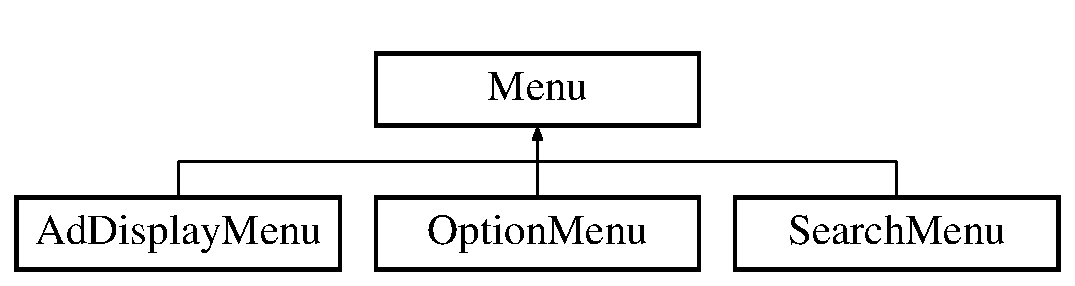
\includegraphics[height=2.000000cm]{class_menu}
\end{center}
\end{figure}
\subsection*{Public Member Functions}
\begin{DoxyCompactItemize}
\item 
\hypertarget{class_menu_a8abee3b9e053fca19f831dd776bd99d1}{}{\bfseries Menu} (\hyperlink{class_data}{Data} $\ast$data, unsigned int height, unsigned int width)\label{class_menu_a8abee3b9e053fca19f831dd776bd99d1}

\item 
\hypertarget{class_menu_aaadfa629cab782a6087766f4fc7b19a6}{}{\bfseries Menu} (\hyperlink{class_data}{Data} $\ast$data, unsigned int height, unsigned int width, char border\+Char)\label{class_menu_aaadfa629cab782a6087766f4fc7b19a6}

\item 
\hypertarget{class_menu_aa0503578e77400a5609f039ed62d44e7}{}void {\bfseries set\+Border\+Char} (char border\+Char)\label{class_menu_aa0503578e77400a5609f039ed62d44e7}

\item 
\hypertarget{class_menu_afdd6e6b09535ca48838c22d5a753dcfc}{}char {\bfseries get\+Border\+Char} ()\label{class_menu_afdd6e6b09535ca48838c22d5a753dcfc}

\item 
\hypertarget{class_menu_ae1857de4af042320041da50debf81709}{}virtual void {\bfseries print} ()=0\label{class_menu_ae1857de4af042320041da50debf81709}

\item 
\hypertarget{class_menu_af71cfef966c0dfd5ecf5d585ddb16514}{}virtual void {\bfseries create\+Menu} ()=0\label{class_menu_af71cfef966c0dfd5ecf5d585ddb16514}

\end{DoxyCompactItemize}
\subsection*{Protected Attributes}
\begin{DoxyCompactItemize}
\item 
\hypertarget{class_menu_a912c40f15f93092412c8d6204c0f8788}{}char {\bfseries border\+Char}\label{class_menu_a912c40f15f93092412c8d6204c0f8788}

\item 
\hypertarget{class_menu_a84dd6e7e6b263601781683951687bf42}{}unsigned int {\bfseries height}\label{class_menu_a84dd6e7e6b263601781683951687bf42}

\item 
\hypertarget{class_menu_a934c7679ed1575cc9924919b9b3eccb1}{}unsigned int {\bfseries width}\label{class_menu_a934c7679ed1575cc9924919b9b3eccb1}

\item 
\hypertarget{class_menu_a572349c0905151704d7cea8e82097e5f}{}unsigned int {\bfseries top\+Margin}\label{class_menu_a572349c0905151704d7cea8e82097e5f}

\item 
\hypertarget{class_menu_acabd9ee2058f2b5cd3bf64903f53d4de}{}unsigned int {\bfseries left\+Margin}\label{class_menu_acabd9ee2058f2b5cd3bf64903f53d4de}

\item 
\hypertarget{class_menu_a3914261df4f4fbadd9c0a854a5f42b0b}{}\hyperlink{class_data}{Data} $\ast$ {\bfseries data}\label{class_menu_a3914261df4f4fbadd9c0a854a5f42b0b}

\end{DoxyCompactItemize}


The documentation for this class was generated from the following files\+:\begin{DoxyCompactItemize}
\item 
O\+L\+Z/src/class/menu/menu.\+h\item 
O\+L\+Z/src/class/menu/menu.\+cpp\end{DoxyCompactItemize}

\hypertarget{class_option_menu}{}\section{Option\+Menu Class Reference}
\label{class_option_menu}\index{Option\+Menu@{Option\+Menu}}
Inheritance diagram for Option\+Menu\+:\begin{figure}[H]
\begin{center}
\leavevmode
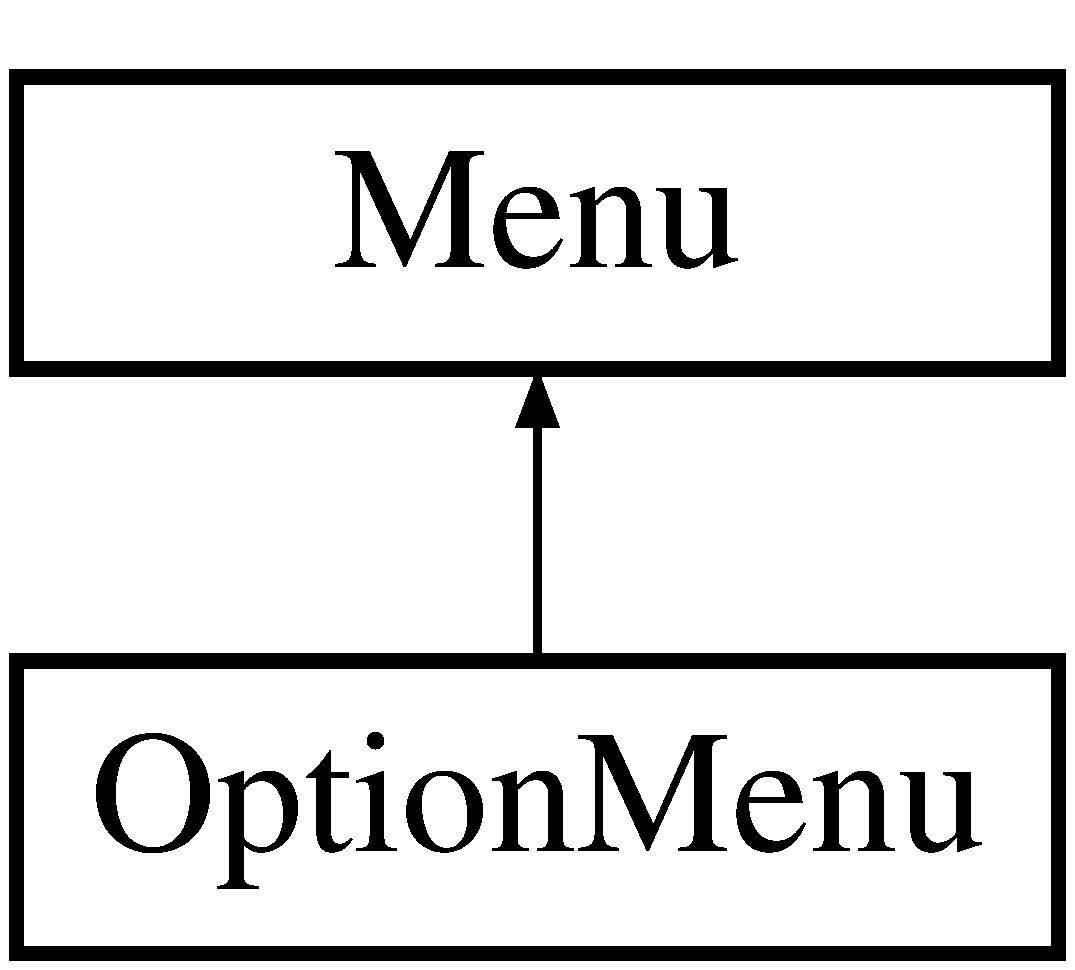
\includegraphics[height=2.000000cm]{class_option_menu}
\end{center}
\end{figure}
\subsection*{Public Member Functions}
\begin{DoxyCompactItemize}
\item 
\hypertarget{class_option_menu_a76889e484d801886f5d48180e4f64a31}{}{\bfseries Option\+Menu} (\hyperlink{class_data}{Data} $\ast$data, unsigned int height=20, unsigned int width=75, char border\+Char= \textquotesingle{}\#\textquotesingle{})\label{class_option_menu_a76889e484d801886f5d48180e4f64a31}

\item 
\hypertarget{class_option_menu_a753b91d8c99330c962d6ecbe520800d2}{}void {\bfseries print} ()\label{class_option_menu_a753b91d8c99330c962d6ecbe520800d2}

\item 
\hypertarget{class_option_menu_a82ce2285fb79bec7073b5358648f19b6}{}void {\bfseries add\+Option} (string name, void($\ast$function)(\hyperlink{class_data}{Data} $\ast$data))\label{class_option_menu_a82ce2285fb79bec7073b5358648f19b6}

\item 
\hypertarget{class_option_menu_a30620df0e9871ce3bbdccf3cb094785f}{}void {\bfseries create\+Menu} ()\label{class_option_menu_a30620df0e9871ce3bbdccf3cb094785f}

\end{DoxyCompactItemize}
\subsection*{Additional Inherited Members}


The documentation for this class was generated from the following files\+:\begin{DoxyCompactItemize}
\item 
O\+L\+Z/src/class/menu/option\+Menu/option\+Menu.\+h\item 
O\+L\+Z/src/class/menu/option\+Menu/option\+Menu.\+cpp\end{DoxyCompactItemize}

\hypertarget{class_purchase}{}\section{Purchase Class Reference}
\label{class_purchase}\index{Purchase@{Purchase}}
Inheritance diagram for Purchase\+:\begin{figure}[H]
\begin{center}
\leavevmode
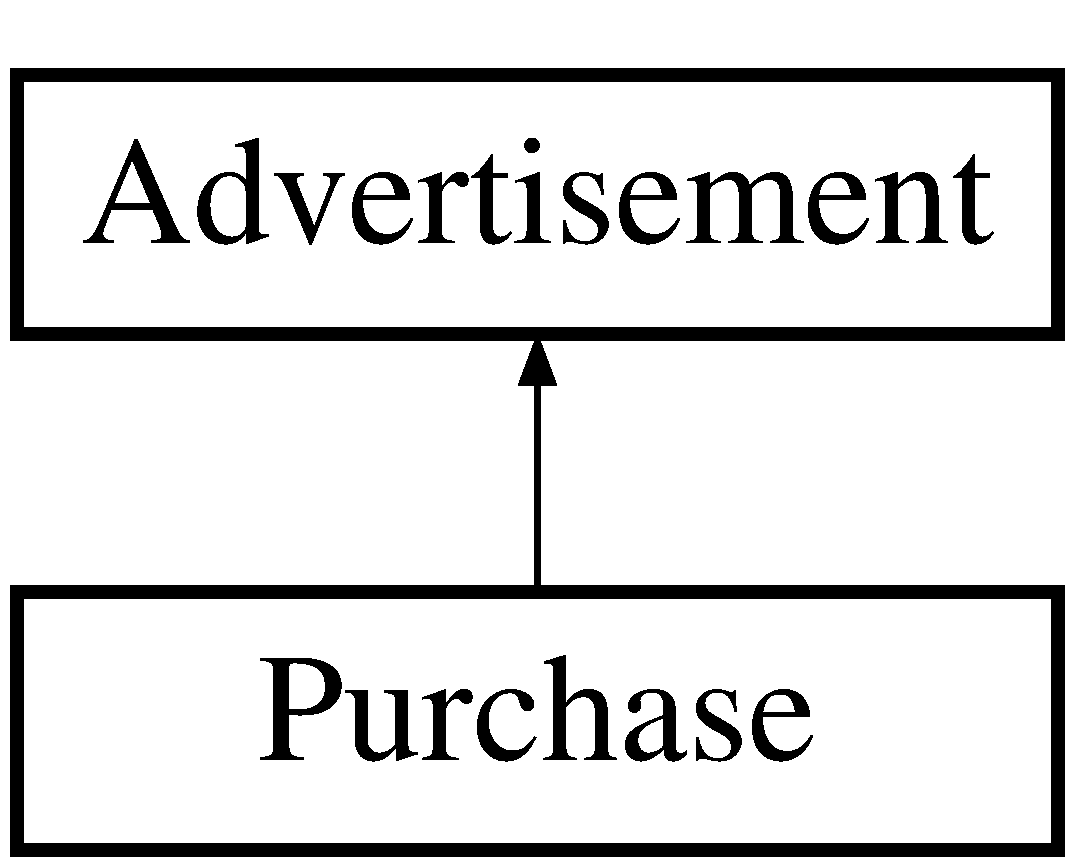
\includegraphics[height=2.000000cm]{class_purchase}
\end{center}
\end{figure}
\subsection*{Public Member Functions}
\begin{DoxyCompactItemize}
\item 
\hypertarget{class_purchase_a5603b3428060205ce26e45441f37d560}{}{\bfseries Purchase} (\hyperlink{class_user}{User} $\ast$owner, string title, Category category, string description)\label{class_purchase_a5603b3428060205ce26e45441f37d560}

\end{DoxyCompactItemize}


The documentation for this class was generated from the following files\+:\begin{DoxyCompactItemize}
\item 
O\+L\+Z/src/class/advertisement/purchase/\hyperlink{purchase_8h}{purchase.\+h}\item 
O\+L\+Z/src/class/advertisement/purchase/\hyperlink{purchase_8cpp}{purchase.\+cpp}\end{DoxyCompactItemize}

\hypertarget{class_sale}{}\section{Sale Class Reference}
\label{class_sale}\index{Sale@{Sale}}


\hyperlink{class_sale}{Sale} class.  




{\ttfamily \#include $<$sale.\+h$>$}

Inheritance diagram for Sale\+:\begin{figure}[H]
\begin{center}
\leavevmode
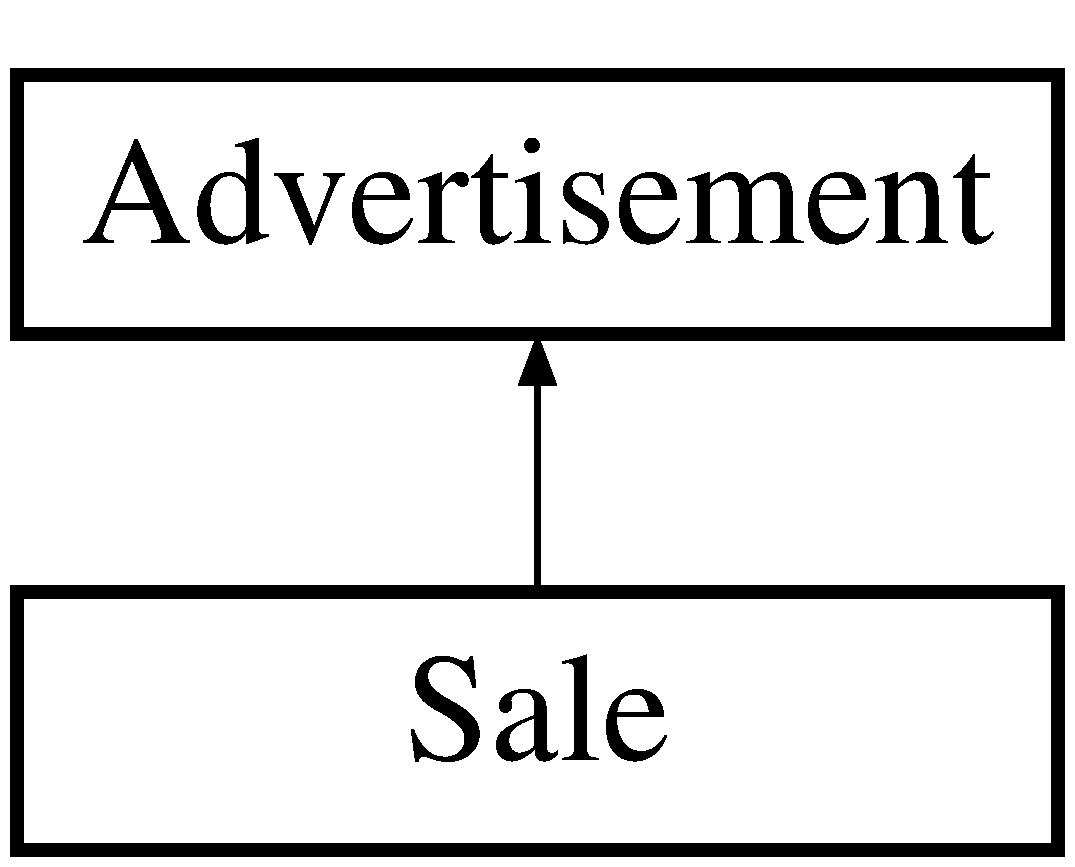
\includegraphics[height=2.000000cm]{class_sale}
\end{center}
\end{figure}
\subsection*{Public Member Functions}
\begin{DoxyCompactItemize}
\item 
\hyperlink{class_sale_ae5f5658a042eaaa8c080c1282d79f9ae}{Sale} (\hyperlink{class_user}{User} $\ast$owner, string title, Category category, string description, Condition product\+Condition)
\begin{DoxyCompactList}\small\item\em \hyperlink{class_sale}{Sale} constructor. \end{DoxyCompactList}\end{DoxyCompactItemize}


\subsection{Detailed Description}
\hyperlink{class_sale}{Sale} class. 

\subsection{Constructor \& Destructor Documentation}
\hypertarget{class_sale_ae5f5658a042eaaa8c080c1282d79f9ae}{}\index{Sale@{Sale}!Sale@{Sale}}
\index{Sale@{Sale}!Sale@{Sale}}
\subsubsection[{Sale(\+User $\ast$owner, string title, Category category, string description, Condition product\+Condition)}]{\setlength{\rightskip}{0pt plus 5cm}Sale\+::\+Sale (
\begin{DoxyParamCaption}
\item[{{\bf User} $\ast$}]{owner, }
\item[{string}]{title, }
\item[{Category}]{category, }
\item[{string}]{description, }
\item[{Condition}]{product\+Condition}
\end{DoxyParamCaption}
)}\label{class_sale_ae5f5658a042eaaa8c080c1282d79f9ae}


\hyperlink{class_sale}{Sale} constructor. 


\begin{DoxyParams}{Parameters}
{\em owner} & Pointer to advertisement owner \\
\hline
{\em title} & \hyperlink{class_advertisement}{Advertisement} title \\
\hline
{\em category} & \hyperlink{class_advertisement}{Advertisement} category \\
\hline
{\em description} & \hyperlink{class_advertisement}{Advertisement} description \\
\hline
{\em product\+Condition} & Product condition \\
\hline
\end{DoxyParams}


The documentation for this class was generated from the following files\+:\begin{DoxyCompactItemize}
\item 
O\+L\+Z/src/class/advertisement/sale/\hyperlink{sale_8h}{sale.\+h}\item 
O\+L\+Z/src/class/advertisement/sale/\hyperlink{sale_8cpp}{sale.\+cpp}\end{DoxyCompactItemize}

\hypertarget{class_search_menu}{}\section{Search\+Menu Class Reference}
\label{class_search_menu}\index{Search\+Menu@{Search\+Menu}}


\hyperlink{class_search_menu}{Search\+Menu} class.  




{\ttfamily \#include $<$search\+Menu.\+h$>$}

Inheritance diagram for Search\+Menu\+:\begin{figure}[H]
\begin{center}
\leavevmode
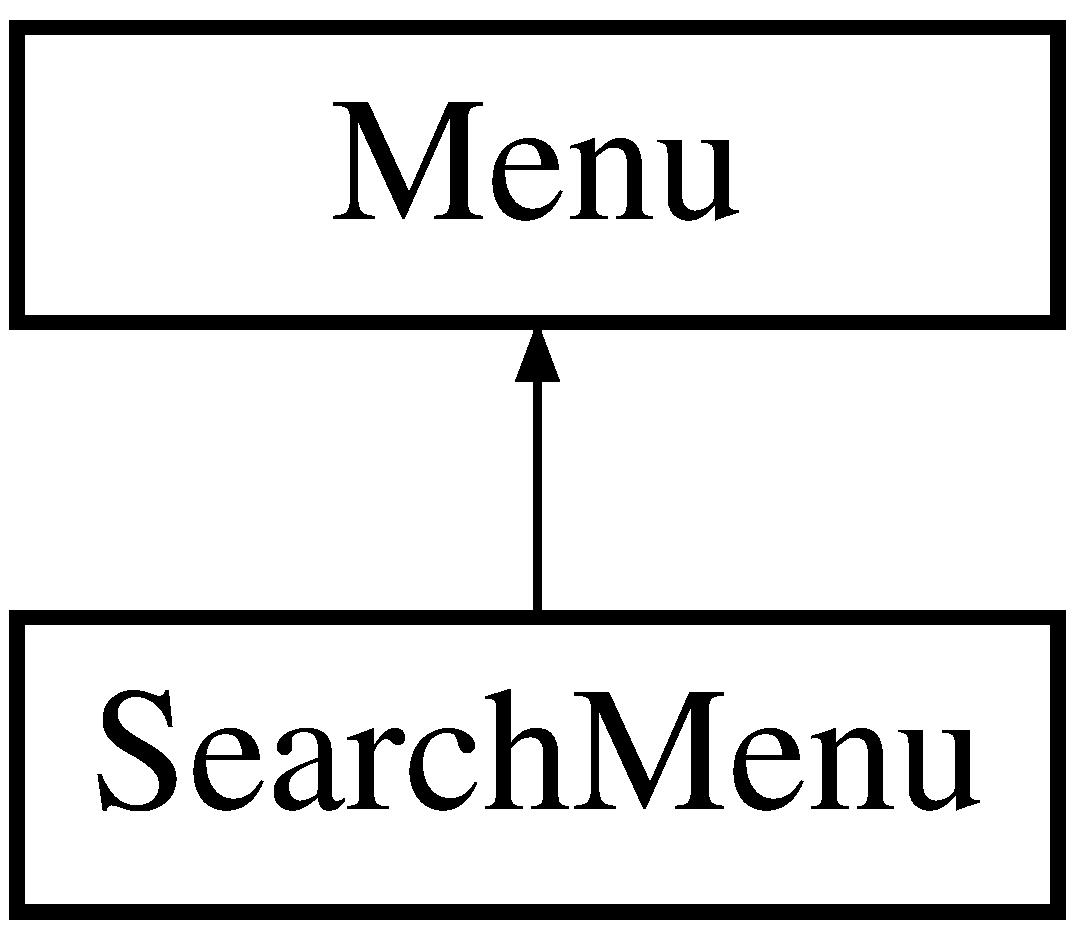
\includegraphics[height=2.000000cm]{class_search_menu}
\end{center}
\end{figure}
\subsection*{Public Member Functions}
\begin{DoxyCompactItemize}
\item 
\hyperlink{class_search_menu_ae0e28277ac4fea08c1f09b9fa502919f}{Search\+Menu} (\hyperlink{class_data}{Data} $\ast$\hyperlink{class_menu_a3914261df4f4fbadd9c0a854a5f42b0b}{data}, vector$<$ \hyperlink{class_advertisement}{Advertisement} $\ast$ $>$ \&results, unsigned int \hyperlink{class_menu_a84dd6e7e6b263601781683951687bf42}{height}=20, unsigned int \hyperlink{class_menu_a934c7679ed1575cc9924919b9b3eccb1}{width}=75, char \hyperlink{class_menu_a912c40f15f93092412c8d6204c0f8788}{border\+Char}= \textquotesingle{}\#\textquotesingle{})
\begin{DoxyCompactList}\small\item\em Constructor for \hyperlink{class_search_menu}{Search\+Menu} class. \end{DoxyCompactList}\item 
void \hyperlink{class_search_menu_a506fce847fc8201ccc63d3fbc2ede3b8}{set\+Ads\+Per\+Page} (unsigned int ads\+Per\+Page)
\begin{DoxyCompactList}\small\item\em Sets ads per page. \end{DoxyCompactList}\item 
unsigned int \hyperlink{class_search_menu_a39156ea5dcb600c0bf12eadc503f7268}{get\+Ads\+Per\+Page} ()
\begin{DoxyCompactList}\small\item\em Gets ads per page. \end{DoxyCompactList}\item 
\hypertarget{class_search_menu_a4fbc2741c5d72f4fe7473e5de5a5d14e}{}void \hyperlink{class_search_menu_a4fbc2741c5d72f4fe7473e5de5a5d14e}{print} ()\label{class_search_menu_a4fbc2741c5d72f4fe7473e5de5a5d14e}

\begin{DoxyCompactList}\small\item\em Prints menu to screen. \end{DoxyCompactList}\item 
\hypertarget{class_search_menu_a97f499b313e88142590aa51c2ef82f3d}{}void \hyperlink{class_search_menu_a97f499b313e88142590aa51c2ef82f3d}{create\+Menu} ()\label{class_search_menu_a97f499b313e88142590aa51c2ef82f3d}

\begin{DoxyCompactList}\small\item\em Handles user interaction. \end{DoxyCompactList}\end{DoxyCompactItemize}
\subsection*{Additional Inherited Members}


\subsection{Detailed Description}
\hyperlink{class_search_menu}{Search\+Menu} class. 

\subsection{Constructor \& Destructor Documentation}
\hypertarget{class_search_menu_ae0e28277ac4fea08c1f09b9fa502919f}{}\index{Search\+Menu@{Search\+Menu}!Search\+Menu@{Search\+Menu}}
\index{Search\+Menu@{Search\+Menu}!Search\+Menu@{Search\+Menu}}
\subsubsection[{Search\+Menu(\+Data $\ast$data, vector$<$ Advertisement $\ast$ $>$ \&results, unsigned int height=20, unsigned int width=75, char border\+Char= \textquotesingle{}\#\textquotesingle{})}]{\setlength{\rightskip}{0pt plus 5cm}Search\+Menu\+::\+Search\+Menu (
\begin{DoxyParamCaption}
\item[{{\bf Data} $\ast$}]{data, }
\item[{vector$<$ {\bf Advertisement} $\ast$ $>$ \&}]{results, }
\item[{unsigned int}]{height = {\ttfamily 20}, }
\item[{unsigned int}]{width = {\ttfamily 75}, }
\item[{char}]{border\+Char = {\ttfamily \textquotesingle{}\#\textquotesingle{}}}
\end{DoxyParamCaption}
)}\label{class_search_menu_ae0e28277ac4fea08c1f09b9fa502919f}


Constructor for \hyperlink{class_search_menu}{Search\+Menu} class. 


\begin{DoxyParams}{Parameters}
{\em data} & \hyperlink{class_data}{Data} \\
\hline
{\em results} & Results to display \\
\hline
{\em height} & \hyperlink{class_menu}{Menu} height \\
\hline
{\em width} & \hyperlink{class_menu}{Menu} width \\
\hline
{\em border\+Char} & Border character \\
\hline
\end{DoxyParams}


\subsection{Member Function Documentation}
\hypertarget{class_search_menu_a39156ea5dcb600c0bf12eadc503f7268}{}\index{Search\+Menu@{Search\+Menu}!get\+Ads\+Per\+Page@{get\+Ads\+Per\+Page}}
\index{get\+Ads\+Per\+Page@{get\+Ads\+Per\+Page}!Search\+Menu@{Search\+Menu}}
\subsubsection[{get\+Ads\+Per\+Page()}]{\setlength{\rightskip}{0pt plus 5cm}unsigned int Search\+Menu\+::get\+Ads\+Per\+Page (
\begin{DoxyParamCaption}
{}
\end{DoxyParamCaption}
)}\label{class_search_menu_a39156ea5dcb600c0bf12eadc503f7268}


Gets ads per page. 

\begin{DoxyReturn}{Returns}
Returns ads per page 
\end{DoxyReturn}
\hypertarget{class_search_menu_a506fce847fc8201ccc63d3fbc2ede3b8}{}\index{Search\+Menu@{Search\+Menu}!set\+Ads\+Per\+Page@{set\+Ads\+Per\+Page}}
\index{set\+Ads\+Per\+Page@{set\+Ads\+Per\+Page}!Search\+Menu@{Search\+Menu}}
\subsubsection[{set\+Ads\+Per\+Page(unsigned int ads\+Per\+Page)}]{\setlength{\rightskip}{0pt plus 5cm}void Search\+Menu\+::set\+Ads\+Per\+Page (
\begin{DoxyParamCaption}
\item[{unsigned int}]{ads\+Per\+Page}
\end{DoxyParamCaption}
)}\label{class_search_menu_a506fce847fc8201ccc63d3fbc2ede3b8}


Sets ads per page. 


\begin{DoxyParams}{Parameters}
{\em ads\+Per\+Page} & Advertisements per page \\
\hline
\end{DoxyParams}


The documentation for this class was generated from the following files\+:\begin{DoxyCompactItemize}
\item 
O\+L\+Z/src/class/menu/search\+Menu/\hyperlink{search_menu_8h}{search\+Menu.\+h}\item 
O\+L\+Z/src/class/menu/search\+Menu/\hyperlink{search_menu_8cpp}{search\+Menu.\+cpp}\end{DoxyCompactItemize}

\hypertarget{class_user}{}\section{User Class Reference}
\label{class_user}\index{User@{User}}
\subsection*{Public Member Functions}
\begin{DoxyCompactItemize}
\item 
\hypertarget{class_user_a670870b549b3675f2ebcc7045f89cd1f}{}{\bfseries User} (string email, string password, string name, string phone\+Number, \hyperlink{class_date}{Date} sign\+Up\+Date, \hyperlink{class_location}{Location} location)\label{class_user_a670870b549b3675f2ebcc7045f89cd1f}

\item 
\hypertarget{class_user_a55fbba82f16e683eba80f23d09d49e06}{}{\bfseries User} (string email, string password, string name, string phone\+Number, \hyperlink{class_date}{Date} sign\+Up\+Date, string location)\label{class_user_a55fbba82f16e683eba80f23d09d49e06}

\item 
\hypertarget{class_user_af75d18fdc45ac9fba9911815b78b7daa}{}bool {\bfseries sign\+In} (string password) const \label{class_user_af75d18fdc45ac9fba9911815b78b7daa}

\item 
\hypertarget{class_user_ac8a15550f3596a7ef13eb31b82a8ecf6}{}string {\bfseries get\+Email} () const \label{class_user_ac8a15550f3596a7ef13eb31b82a8ecf6}

\item 
\hypertarget{class_user_a2b2a3d00d303affb4f5674bc9788db52}{}string {\bfseries get\+Name} () const \label{class_user_a2b2a3d00d303affb4f5674bc9788db52}

\item 
\hypertarget{class_user_a4d59412a7d7411dd8c8127adc9e80fae}{}string {\bfseries get\+Phone\+Number} () const \label{class_user_a4d59412a7d7411dd8c8127adc9e80fae}

\item 
\hypertarget{class_user_a7c2072cbf540ae1bd47992b40783843c}{}\hyperlink{class_location}{Location} {\bfseries get\+Location} () const \label{class_user_a7c2072cbf540ae1bd47992b40783843c}

\item 
\hypertarget{class_user_a7185d303044e8dbb683b717228e2560d}{}string {\bfseries get\+Location\+String} () const \label{class_user_a7185d303044e8dbb683b717228e2560d}

\item 
\hypertarget{class_user_aa3bb1db20bfdae4ae26f8e5b84360f45}{}void {\bfseries remove\+Advertisement} (unsigned int id)\label{class_user_aa3bb1db20bfdae4ae26f8e5b84360f45}

\end{DoxyCompactItemize}
\subsection*{Protected Attributes}
\begin{DoxyCompactItemize}
\item 
\hypertarget{class_user_a9a78e0f9ab50c5d9d3041d1d90acd4d8}{}vector$<$ \hyperlink{class_advertisement}{Advertisement} $\ast$ $>$ {\bfseries advertisements}\label{class_user_a9a78e0f9ab50c5d9d3041d1d90acd4d8}

\item 
\hypertarget{class_user_a2d678acd22b533660b4b7d8404961f14}{}string {\bfseries email}\label{class_user_a2d678acd22b533660b4b7d8404961f14}

\item 
\hypertarget{class_user_ab537b9a55bc7d7fcafcdf8e53d085e67}{}string {\bfseries password}\label{class_user_ab537b9a55bc7d7fcafcdf8e53d085e67}

\item 
\hypertarget{class_user_a643f85779a4693855c171c396f49e515}{}string {\bfseries name}\label{class_user_a643f85779a4693855c171c396f49e515}

\item 
\hypertarget{class_user_a727ba647fe019be6fa9c03308d60da9e}{}string {\bfseries phone\+Number}\label{class_user_a727ba647fe019be6fa9c03308d60da9e}

\item 
\hypertarget{class_user_ab508f13f113618c508641e7f47932cc9}{}\hyperlink{class_date}{Date} {\bfseries sign\+Up\+Date}\label{class_user_ab508f13f113618c508641e7f47932cc9}

\item 
\hypertarget{class_user_a1c8e68a346c8a47d8cf0e75356c66562}{}\hyperlink{class_location}{Location} {\bfseries location}\label{class_user_a1c8e68a346c8a47d8cf0e75356c66562}

\end{DoxyCompactItemize}
\subsection*{Friends}
\begin{DoxyCompactItemize}
\item 
\hypertarget{class_user_a450594b5d214c6f0e33a61a070d77422}{}istream \& {\bfseries operator$>$$>$} (istream \&in, \hyperlink{class_user}{User} user)\label{class_user_a450594b5d214c6f0e33a61a070d77422}

\end{DoxyCompactItemize}


The documentation for this class was generated from the following files\+:\begin{DoxyCompactItemize}
\item 
O\+L\+Z/src/class/user/user.\+h\item 
O\+L\+Z/src/class/user/user.\+cpp\end{DoxyCompactItemize}

\chapter{File Documentation}
\hypertarget{advertisement_8cpp}{}\section{O\+L\+Z/src/class/advertisement/advertisement.cpp File Reference}
\label{advertisement_8cpp}\index{O\+L\+Z/src/class/advertisement/advertisement.\+cpp@{O\+L\+Z/src/class/advertisement/advertisement.\+cpp}}


Code for class \hyperlink{class_advertisement}{Advertisement}.  


{\ttfamily \#include \char`\"{}advertisement.\+h\char`\"{}}\\*
{\ttfamily \#include \char`\"{}../menu/ad\+Display\+Menu/ad\+Display\+Menu.\+h\char`\"{}}\\*
{\ttfamily \#include $<$iostream$>$}\\*
{\ttfamily \#include $<$sstream$>$}\\*
\subsection*{Functions}
\begin{DoxyCompactItemize}
\item 
ostream \& \hyperlink{advertisement_8cpp_af6ba8e9ebe3c64e17263cbbcaa8bbb59}{operator$<$$<$} (ostream \&out, \hyperlink{class_advertisement}{Advertisement} \&ad)
\item 
istream \& \hyperlink{advertisement_8cpp_a5180e86255ebd01c83666f431b910bb4}{operator$>$$>$} (istream \&in, \hyperlink{class_advertisement}{Advertisement} \&ad)
\end{DoxyCompactItemize}


\subsection{Detailed Description}
Code for class \hyperlink{class_advertisement}{Advertisement}. 



\subsection{Function Documentation}
\hypertarget{advertisement_8cpp_af6ba8e9ebe3c64e17263cbbcaa8bbb59}{}\index{advertisement.\+cpp@{advertisement.\+cpp}!operator$<$$<$@{operator$<$$<$}}
\index{operator$<$$<$@{operator$<$$<$}!advertisement.\+cpp@{advertisement.\+cpp}}
\subsubsection[{operator$<$$<$(ostream \&out, Advertisement \&ad)}]{\setlength{\rightskip}{0pt plus 5cm}ostream\& operator$<$$<$ (
\begin{DoxyParamCaption}
\item[{ostream \&}]{out, }
\item[{{\bf Advertisement} \&}]{ad}
\end{DoxyParamCaption}
)}\label{advertisement_8cpp_af6ba8e9ebe3c64e17263cbbcaa8bbb59}

\begin{DoxyParams}{Parameters}
{\em out} & Out stream \\
\hline
{\em ad} & Reference to advertisement to print\\
\hline
\end{DoxyParams}
\begin{DoxyReturn}{Returns}
Returns out stream 
\end{DoxyReturn}
\hypertarget{advertisement_8cpp_a5180e86255ebd01c83666f431b910bb4}{}\index{advertisement.\+cpp@{advertisement.\+cpp}!operator$>$$>$@{operator$>$$>$}}
\index{operator$>$$>$@{operator$>$$>$}!advertisement.\+cpp@{advertisement.\+cpp}}
\subsubsection[{operator$>$$>$(istream \&in, Advertisement \&ad)}]{\setlength{\rightskip}{0pt plus 5cm}istream\& operator$>$$>$ (
\begin{DoxyParamCaption}
\item[{istream \&}]{in, }
\item[{{\bf Advertisement} \&}]{ad}
\end{DoxyParamCaption}
)}\label{advertisement_8cpp_a5180e86255ebd01c83666f431b910bb4}

\begin{DoxyParams}{Parameters}
{\em in} & In stream \\
\hline
{\em ad} & Reference to advertisement to write on\\
\hline
\end{DoxyParams}
\begin{DoxyReturn}{Returns}
Returns in stream 
\end{DoxyReturn}

\hypertarget{advertisement_8h}{}\section{O\+L\+Z/src/class/advertisement/advertisement.h File Reference}
\label{advertisement_8h}\index{O\+L\+Z/src/class/advertisement/advertisement.\+h@{O\+L\+Z/src/class/advertisement/advertisement.\+h}}


Header file for class \hyperlink{class_advertisement}{Advertisement}.  


{\ttfamily \#include $<$string$>$}\\*
{\ttfamily \#include $<$vector$>$}\\*
{\ttfamily \#include \char`\"{}../../enums.\+h\char`\"{}}\\*
{\ttfamily \#include \char`\"{}../date/date.\+h\char`\"{}}\\*
{\ttfamily \#include \char`\"{}../user/user.\+h\char`\"{}}\\*
\subsection*{Classes}
\begin{DoxyCompactItemize}
\item 
class \hyperlink{class_advertisement}{Advertisement}
\begin{DoxyCompactList}\small\item\em \hyperlink{class_advertisement}{Advertisement} class. \end{DoxyCompactList}\end{DoxyCompactItemize}


\subsection{Detailed Description}
Header file for class \hyperlink{class_advertisement}{Advertisement}. 


\hypertarget{purchase_8cpp}{}\section{O\+L\+Z/src/class/advertisement/purchase/purchase.cpp File Reference}
\label{purchase_8cpp}\index{O\+L\+Z/src/class/advertisement/purchase/purchase.\+cpp@{O\+L\+Z/src/class/advertisement/purchase/purchase.\+cpp}}


Code for class \hyperlink{class_purchase}{Purchase}.  


{\ttfamily \#include \char`\"{}purchase.\+h\char`\"{}}\\*
{\ttfamily \#include \char`\"{}../advertisement.\+h\char`\"{}}\\*


\subsection{Detailed Description}
Code for class \hyperlink{class_purchase}{Purchase}. 


\hypertarget{purchase_8h}{}\section{O\+L\+Z/src/class/advertisement/purchase/purchase.h File Reference}
\label{purchase_8h}\index{O\+L\+Z/src/class/advertisement/purchase/purchase.\+h@{O\+L\+Z/src/class/advertisement/purchase/purchase.\+h}}


Header file for class \hyperlink{class_purchase}{Purchase}.  


{\ttfamily \#include \char`\"{}../advertisement.\+h\char`\"{}}\\*
\subsection*{Classes}
\begin{DoxyCompactItemize}
\item 
class \hyperlink{class_purchase}{Purchase}
\end{DoxyCompactItemize}


\subsection{Detailed Description}
Header file for class \hyperlink{class_purchase}{Purchase}. 


\hypertarget{sale_8cpp}{}\section{O\+L\+Z/src/class/advertisement/sale/sale.cpp File Reference}
\label{sale_8cpp}\index{O\+L\+Z/src/class/advertisement/sale/sale.\+cpp@{O\+L\+Z/src/class/advertisement/sale/sale.\+cpp}}


Code for class \hyperlink{class_sale}{Sale}.  


{\ttfamily \#include \char`\"{}sale.\+h\char`\"{}}\\*
{\ttfamily \#include \char`\"{}../../menu/ad\+Display\+Menu/ad\+Display\+Menu.\+h\char`\"{}}\\*
{\ttfamily \#include \char`\"{}../../../enums.\+h\char`\"{}}\\*
{\ttfamily \#include $<$iostream$>$}\\*


\subsection{Detailed Description}
Code for class \hyperlink{class_sale}{Sale}. 


\hypertarget{sale_8h}{}\section{O\+L\+Z/src/class/advertisement/sale/sale.h File Reference}
\label{sale_8h}\index{O\+L\+Z/src/class/advertisement/sale/sale.\+h@{O\+L\+Z/src/class/advertisement/sale/sale.\+h}}


Header file for class \hyperlink{class_sale}{Sale}.  


{\ttfamily \#include \char`\"{}../../../enums.\+h\char`\"{}}\\*
{\ttfamily \#include \char`\"{}../advertisement.\+h\char`\"{}}\\*
\subsection*{Classes}
\begin{DoxyCompactItemize}
\item 
class \hyperlink{class_sale}{Sale}
\begin{DoxyCompactList}\small\item\em \hyperlink{class_sale}{Sale} class. \end{DoxyCompactList}\end{DoxyCompactItemize}


\subsection{Detailed Description}
Header file for class \hyperlink{class_sale}{Sale}. 


\hypertarget{data_8cpp}{}\section{O\+L\+Z/src/class/data/data.cpp File Reference}
\label{data_8cpp}\index{O\+L\+Z/src/class/data/data.\+cpp@{O\+L\+Z/src/class/data/data.\+cpp}}


Code for class \hyperlink{class_data}{Data}.  


{\ttfamily \#include \char`\"{}data.\+h\char`\"{}}\\*
{\ttfamily \#include \char`\"{}../../sequential\+Search.\+h\char`\"{}}\\*
{\ttfamily \#include \char`\"{}../advertisement/purchase/purchase.\+h\char`\"{}}\\*
{\ttfamily \#include \char`\"{}../../menus.\+h\char`\"{}}\\*
{\ttfamily \#include $<$fstream$>$}\\*
{\ttfamily \#include $<$iostream$>$}\\*
{\ttfamily \#include $<$sstream$>$}\\*


\subsection{Detailed Description}
Code for class \hyperlink{class_data}{Data}. 


\hypertarget{data_8h}{}\section{O\+L\+Z/src/class/data/data.h File Reference}
\label{data_8h}\index{O\+L\+Z/src/class/data/data.\+h@{O\+L\+Z/src/class/data/data.\+h}}


Header file for class \hyperlink{class_data}{Data}.  


{\ttfamily \#include $<$vector$>$}\\*
{\ttfamily \#include \char`\"{}../user/user.\+h\char`\"{}}\\*
\subsection*{Classes}
\begin{DoxyCompactItemize}
\item 
class \hyperlink{class_data}{Data}
\begin{DoxyCompactList}\small\item\em \hyperlink{class_user}{User} and \hyperlink{class_advertisement}{Advertisement} data class. \end{DoxyCompactList}\end{DoxyCompactItemize}


\subsection{Detailed Description}
Header file for class \hyperlink{class_data}{Data}. 


\hypertarget{date_8cpp}{}\section{O\+L\+Z/src/class/date/date.cpp File Reference}
\label{date_8cpp}\index{O\+L\+Z/src/class/date/date.\+cpp@{O\+L\+Z/src/class/date/date.\+cpp}}


Code for class \hyperlink{class_date}{Date}.  


{\ttfamily \#include \char`\"{}date.\+h\char`\"{}}\\*
{\ttfamily \#include $<$sstream$>$}\\*
{\ttfamily \#include $<$stdlib.\+h$>$}\\*
{\ttfamily \#include $<$stdexcept$>$}\\*
{\ttfamily \#include $<$iostream$>$}\\*
\subsection*{Functions}
\begin{DoxyCompactItemize}
\item 
ostream \& \hyperlink{date_8cpp_a5c29d00ecf33e6d232a410f1f3d6eb70}{operator$<$$<$} (ostream \&out, const \hyperlink{class_date}{Date} \&date)
\end{DoxyCompactItemize}


\subsection{Detailed Description}
Code for class \hyperlink{class_date}{Date}. 



\subsection{Function Documentation}
\hypertarget{date_8cpp_a5c29d00ecf33e6d232a410f1f3d6eb70}{}\index{date.\+cpp@{date.\+cpp}!operator$<$$<$@{operator$<$$<$}}
\index{operator$<$$<$@{operator$<$$<$}!date.\+cpp@{date.\+cpp}}
\subsubsection[{operator$<$$<$(ostream \&out, const Date \&date)}]{\setlength{\rightskip}{0pt plus 5cm}ostream\& operator$<$$<$ (
\begin{DoxyParamCaption}
\item[{ostream \&}]{out, }
\item[{const {\bf Date} \&}]{date}
\end{DoxyParamCaption}
)}\label{date_8cpp_a5c29d00ecf33e6d232a410f1f3d6eb70}

\begin{DoxyParams}{Parameters}
{\em out} & Out stream \\
\hline
{\em date} & \hyperlink{class_date}{Date} to be printed\\
\hline
\end{DoxyParams}
\begin{DoxyReturn}{Returns}
Returns out stream 
\end{DoxyReturn}

\hypertarget{date_8h}{}\section{O\+L\+Z/src/class/date/date.h File Reference}
\label{date_8h}\index{O\+L\+Z/src/class/date/date.\+h@{O\+L\+Z/src/class/date/date.\+h}}


Header file for class \hyperlink{class_date}{Date}.  


{\ttfamily \#include $<$string$>$}\\*
\subsection*{Classes}
\begin{DoxyCompactItemize}
\item 
class \hyperlink{class_date}{Date}
\begin{DoxyCompactList}\small\item\em \hyperlink{class_date}{Date} class. \end{DoxyCompactList}\end{DoxyCompactItemize}


\subsection{Detailed Description}
Header file for class \hyperlink{class_date}{Date}. 


\hypertarget{location_8cpp}{}\section{O\+L\+Z/src/class/location/location.cpp File Reference}
\label{location_8cpp}\index{O\+L\+Z/src/class/location/location.\+cpp@{O\+L\+Z/src/class/location/location.\+cpp}}


Code for class \hyperlink{class_location}{Location}.  


{\ttfamily \#include \char`\"{}location.\+h\char`\"{}}\\*
\subsection*{Functions}
\begin{DoxyCompactItemize}
\item 
ostream \& \hyperlink{location_8cpp_acbdedd349c06b3c398317f9a9a9d3fe8}{operator$<$$<$} (ostream \&os, const \hyperlink{class_location}{Location} \&location)
\end{DoxyCompactItemize}


\subsection{Detailed Description}
Code for class \hyperlink{class_location}{Location}. 



\subsection{Function Documentation}
\hypertarget{location_8cpp_acbdedd349c06b3c398317f9a9a9d3fe8}{}\index{location.\+cpp@{location.\+cpp}!operator$<$$<$@{operator$<$$<$}}
\index{operator$<$$<$@{operator$<$$<$}!location.\+cpp@{location.\+cpp}}
\subsubsection[{operator$<$$<$(ostream \&os, const Location \&location)}]{\setlength{\rightskip}{0pt plus 5cm}ostream\& operator$<$$<$ (
\begin{DoxyParamCaption}
\item[{ostream \&}]{os, }
\item[{const {\bf Location} \&}]{location}
\end{DoxyParamCaption}
)}\label{location_8cpp_acbdedd349c06b3c398317f9a9a9d3fe8}
\begin{DoxyReturn}{Returns}
Returns output stream 
\end{DoxyReturn}

\hypertarget{location_8h}{}\section{O\+L\+Z/src/class/location/location.h File Reference}
\label{location_8h}\index{O\+L\+Z/src/class/location/location.\+h@{O\+L\+Z/src/class/location/location.\+h}}


Header file for class \hyperlink{class_location}{Location}.  


{\ttfamily \#include $<$string$>$}\\*
\subsection*{Classes}
\begin{DoxyCompactItemize}
\item 
class \hyperlink{class_location}{Location}
\begin{DoxyCompactList}\small\item\em Code for class \hyperlink{class_location}{Location}. A county has many cities; a district has various counties. \end{DoxyCompactList}\end{DoxyCompactItemize}


\subsection{Detailed Description}
Header file for class \hyperlink{class_location}{Location}. 


\hypertarget{ad_display_menu_8cpp}{}\section{O\+L\+Z/src/class/menu/ad\+Display\+Menu/ad\+Display\+Menu.cpp File Reference}
\label{ad_display_menu_8cpp}\index{O\+L\+Z/src/class/menu/ad\+Display\+Menu/ad\+Display\+Menu.\+cpp@{O\+L\+Z/src/class/menu/ad\+Display\+Menu/ad\+Display\+Menu.\+cpp}}


Code for class \hyperlink{class_ad_display_menu}{Ad\+Display\+Menu}.  


{\ttfamily \#include \char`\"{}../../../menus.\+h\char`\"{}}\\*
{\ttfamily \#include \char`\"{}ad\+Display\+Menu.\+h\char`\"{}}\\*
{\ttfamily \#include \char`\"{}../../../enums.\+h\char`\"{}}\\*
{\ttfamily \#include $<$sstream$>$}\\*
{\ttfamily \#include $<$iostream$>$}\\*


\subsection{Detailed Description}
Code for class \hyperlink{class_ad_display_menu}{Ad\+Display\+Menu}. 


\hypertarget{ad_display_menu_8h}{}\section{O\+L\+Z/src/class/menu/ad\+Display\+Menu/ad\+Display\+Menu.h File Reference}
\label{ad_display_menu_8h}\index{O\+L\+Z/src/class/menu/ad\+Display\+Menu/ad\+Display\+Menu.\+h@{O\+L\+Z/src/class/menu/ad\+Display\+Menu/ad\+Display\+Menu.\+h}}


Header file for class \hyperlink{class_ad_display_menu}{Ad\+Display\+Menu}.  


{\ttfamily \#include \char`\"{}../menu.\+h\char`\"{}}\\*
{\ttfamily \#include \char`\"{}../../advertisement/advertisement.\+h\char`\"{}}\\*
\subsection*{Classes}
\begin{DoxyCompactItemize}
\item 
class \hyperlink{class_ad_display_menu}{Ad\+Display\+Menu}
\begin{DoxyCompactList}\small\item\em Code for class \hyperlink{class_ad_display_menu}{Ad\+Display\+Menu}. \end{DoxyCompactList}\end{DoxyCompactItemize}


\subsection{Detailed Description}
Header file for class \hyperlink{class_ad_display_menu}{Ad\+Display\+Menu}. 


\hypertarget{menu_8cpp}{}\section{O\+L\+Z/src/class/menu/menu.cpp File Reference}
\label{menu_8cpp}\index{O\+L\+Z/src/class/menu/menu.\+cpp@{O\+L\+Z/src/class/menu/menu.\+cpp}}


Code for class \hyperlink{class_menu}{Menu}.  


{\ttfamily \#include \char`\"{}menu.\+h\char`\"{}}\\*
{\ttfamily \#include $<$iostream$>$}\\*
{\ttfamily \#include $<$string$>$}\\*
{\ttfamily \#include $<$sstream$>$}\\*


\subsection{Detailed Description}
Code for class \hyperlink{class_menu}{Menu}. 


\hypertarget{menu_8h}{}\section{O\+L\+Z/src/class/menu/menu.h File Reference}
\label{menu_8h}\index{O\+L\+Z/src/class/menu/menu.\+h@{O\+L\+Z/src/class/menu/menu.\+h}}


Header file for class \hyperlink{class_menu}{Menu}.  


{\ttfamily \#include \char`\"{}../data/data.\+h\char`\"{}}\\*
\subsection*{Classes}
\begin{DoxyCompactItemize}
\item 
class \hyperlink{class_menu}{Menu}
\begin{DoxyCompactList}\small\item\em \hyperlink{class_menu}{Menu} class. \end{DoxyCompactList}\end{DoxyCompactItemize}


\subsection{Detailed Description}
Header file for class \hyperlink{class_menu}{Menu}. 


\hypertarget{option_menu_8cpp}{}\section{O\+L\+Z/src/class/menu/option\+Menu/option\+Menu.cpp File Reference}
\label{option_menu_8cpp}\index{O\+L\+Z/src/class/menu/option\+Menu/option\+Menu.\+cpp@{O\+L\+Z/src/class/menu/option\+Menu/option\+Menu.\+cpp}}


Code for class \hyperlink{class_option_menu}{Option\+Menu}.  


{\ttfamily \#include \char`\"{}../../../menus.\+h\char`\"{}}\\*
{\ttfamily \#include \char`\"{}option\+Menu.\+h\char`\"{}}\\*
{\ttfamily \#include $<$exception$>$}\\*
{\ttfamily \#include $<$iostream$>$}\\*
{\ttfamily \#include $<$sstream$>$}\\*


\subsection{Detailed Description}
Code for class \hyperlink{class_option_menu}{Option\+Menu}. 


\hypertarget{option_menu_8h}{}\section{O\+L\+Z/src/class/menu/option\+Menu/option\+Menu.h File Reference}
\label{option_menu_8h}\index{O\+L\+Z/src/class/menu/option\+Menu/option\+Menu.\+h@{O\+L\+Z/src/class/menu/option\+Menu/option\+Menu.\+h}}


Header file for class \hyperlink{class_option_menu}{Option\+Menu}.  


{\ttfamily \#include \char`\"{}../menu.\+h\char`\"{}}\\*
{\ttfamily \#include $<$string$>$}\\*
{\ttfamily \#include $<$utility$>$}\\*
{\ttfamily \#include $<$vector$>$}\\*
\subsection*{Classes}
\begin{DoxyCompactItemize}
\item 
class \hyperlink{class_option_menu}{Option\+Menu}
\begin{DoxyCompactList}\small\item\em \hyperlink{class_option_menu}{Option\+Menu} class. \end{DoxyCompactList}\end{DoxyCompactItemize}


\subsection{Detailed Description}
Header file for class \hyperlink{class_option_menu}{Option\+Menu}. 


\hypertarget{search_menu_8cpp}{}\section{O\+L\+Z/src/class/menu/search\+Menu/search\+Menu.cpp File Reference}
\label{search_menu_8cpp}\index{O\+L\+Z/src/class/menu/search\+Menu/search\+Menu.\+cpp@{O\+L\+Z/src/class/menu/search\+Menu/search\+Menu.\+cpp}}


Code for class \hyperlink{class_search_menu}{Search\+Menu}.  


{\ttfamily \#include \char`\"{}search\+Menu.\+h\char`\"{}}\\*
{\ttfamily \#include \char`\"{}../ad\+Display\+Menu/ad\+Display\+Menu.\+h\char`\"{}}\\*
{\ttfamily \#include \char`\"{}../../../menus.\+h\char`\"{}}\\*
{\ttfamily \#include $<$iostream$>$}\\*
{\ttfamily \#include $<$sstream$>$}\\*
{\ttfamily \#include $<$math.\+h$>$}\\*
{\ttfamily \#include $<$stdlib.\+h$>$}\\*


\subsection{Detailed Description}
Code for class \hyperlink{class_search_menu}{Search\+Menu}. 


\hypertarget{search_menu_8h}{}\section{O\+L\+Z/src/class/menu/search\+Menu/search\+Menu.h File Reference}
\label{search_menu_8h}\index{O\+L\+Z/src/class/menu/search\+Menu/search\+Menu.\+h@{O\+L\+Z/src/class/menu/search\+Menu/search\+Menu.\+h}}


Header file for class \hyperlink{class_search_menu}{Search\+Menu}.  


{\ttfamily \#include \char`\"{}../menu.\+h\char`\"{}}\\*
\subsection*{Classes}
\begin{DoxyCompactItemize}
\item 
class \hyperlink{class_search_menu}{Search\+Menu}
\begin{DoxyCompactList}\small\item\em \hyperlink{class_search_menu}{Search\+Menu} class. \end{DoxyCompactList}\end{DoxyCompactItemize}


\subsection{Detailed Description}
Header file for class \hyperlink{class_search_menu}{Search\+Menu}. 


\hypertarget{user_8cpp}{}\section{O\+L\+Z/src/class/user/user.cpp File Reference}
\label{user_8cpp}\index{O\+L\+Z/src/class/user/user.\+cpp@{O\+L\+Z/src/class/user/user.\+cpp}}


Code for class \hyperlink{class_user}{User}.  


{\ttfamily \#include \char`\"{}user.\+h\char`\"{}}\\*
{\ttfamily \#include \char`\"{}../../sequential\+Search.\+h\char`\"{}}\\*
{\ttfamily \#include \char`\"{}../advertisement/purchase/purchase.\+h\char`\"{}}\\*
{\ttfamily \#include \char`\"{}../advertisement/sale/sale.\+h\char`\"{}}\\*
{\ttfamily \#include \char`\"{}../../enums.\+h\char`\"{}}\\*
{\ttfamily \#include $<$iostream$>$}\\*
{\ttfamily \#include $<$sstream$>$}\\*
\subsection*{Functions}
\begin{DoxyCompactItemize}
\item 
istream \& \hyperlink{user_8cpp_aae624f64cdd1af3b59c2443cffa82494}{operator$>$$>$} (istream \&in, \hyperlink{class_user}{User} \&user)
\item 
ostream \& \hyperlink{user_8cpp_acf1038a8d320684dc3fbdd5e4308e062}{operator$<$$<$} (ostream \&out, const \hyperlink{class_user}{User} \&user)
\end{DoxyCompactItemize}


\subsection{Detailed Description}
Code for class \hyperlink{class_user}{User}. 



\subsection{Function Documentation}
\hypertarget{user_8cpp_acf1038a8d320684dc3fbdd5e4308e062}{}\index{user.\+cpp@{user.\+cpp}!operator$<$$<$@{operator$<$$<$}}
\index{operator$<$$<$@{operator$<$$<$}!user.\+cpp@{user.\+cpp}}
\subsubsection[{operator$<$$<$(ostream \&out, const User \&user)}]{\setlength{\rightskip}{0pt plus 5cm}ostream\& operator$<$$<$ (
\begin{DoxyParamCaption}
\item[{ostream \&}]{out, }
\item[{const {\bf User} \&}]{user}
\end{DoxyParamCaption}
)}\label{user_8cpp_acf1038a8d320684dc3fbdd5e4308e062}

\begin{DoxyParams}{Parameters}
{\em out} & Output file \\
\hline
{\em user} & \hyperlink{class_user}{User} to print\\
\hline
\end{DoxyParams}
\begin{DoxyReturn}{Returns}
Returns out stream 
\end{DoxyReturn}
\hypertarget{user_8cpp_aae624f64cdd1af3b59c2443cffa82494}{}\index{user.\+cpp@{user.\+cpp}!operator$>$$>$@{operator$>$$>$}}
\index{operator$>$$>$@{operator$>$$>$}!user.\+cpp@{user.\+cpp}}
\subsubsection[{operator$>$$>$(istream \&in, User \&user)}]{\setlength{\rightskip}{0pt plus 5cm}istream\& operator$>$$>$ (
\begin{DoxyParamCaption}
\item[{istream \&}]{in, }
\item[{{\bf User} \&}]{user}
\end{DoxyParamCaption}
)}\label{user_8cpp_aae624f64cdd1af3b59c2443cffa82494}
\begin{DoxyReturn}{Returns}
Returns input stream 
\end{DoxyReturn}

\hypertarget{user_8h}{}\section{O\+L\+Z/src/class/user/user.h File Reference}
\label{user_8h}\index{O\+L\+Z/src/class/user/user.\+h@{O\+L\+Z/src/class/user/user.\+h}}


Header file for class \hyperlink{class_user}{User}.  


{\ttfamily \#include $<$string$>$}\\*
{\ttfamily \#include $<$vector$>$}\\*
{\ttfamily \#include \char`\"{}../advertisement/advertisement.\+h\char`\"{}}\\*
{\ttfamily \#include \char`\"{}../date/date.\+h\char`\"{}}\\*
{\ttfamily \#include \char`\"{}../location/location.\+h\char`\"{}}\\*
\subsection*{Classes}
\begin{DoxyCompactItemize}
\item 
class \hyperlink{class_user}{User}
\begin{DoxyCompactList}\small\item\em \hyperlink{class_date}{Date} class. \end{DoxyCompactList}\end{DoxyCompactItemize}


\subsection{Detailed Description}
Header file for class \hyperlink{class_user}{User}. 


\hypertarget{enums_8cpp}{}\section{O\+L\+Z/src/enums.cpp File Reference}
\label{enums_8cpp}\index{O\+L\+Z/src/enums.\+cpp@{O\+L\+Z/src/enums.\+cpp}}


Code for enumerations and their conversion.  


{\ttfamily \#include \char`\"{}enums.\+h\char`\"{}}\\*
\subsection*{Functions}
\begin{DoxyCompactItemize}
\item 
bool \hyperlink{enums_8cpp_adc8f8dd0fdb2eb5da5b08e0737e5befd}{valid\+Category} (string is\+Valid\+Category)
\begin{DoxyCompactList}\small\item\em See if valid\+Category is a valid category then changes the value of category. \end{DoxyCompactList}\item 
Category \hyperlink{enums_8cpp_a88c2d08dec32fa87427679ca28f825e6}{string\+To\+Category} (string \hyperlink{enums_8h_adc8f8dd0fdb2eb5da5b08e0737e5befd}{valid\+Category})
\begin{DoxyCompactList}\small\item\em Changes a string to a category. \end{DoxyCompactList}\item 
string \hyperlink{enums_8cpp_aa1389e4ccfea1de64e309ca65b7a4a71}{category\+To\+String} (Category \hyperlink{enums_8h_adc8f8dd0fdb2eb5da5b08e0737e5befd}{valid\+Category})
\begin{DoxyCompactList}\small\item\em Changes a string to a category. \end{DoxyCompactList}\item 
bool \hyperlink{enums_8cpp_ac44afaa3fb3951470f45296c763b772b}{valid\+Condition} (string is\+Valid\+Condition)
\begin{DoxyCompactList}\small\item\em See if valid\+Category is a valid category then changes the value of category. \end{DoxyCompactList}\item 
Condition \hyperlink{enums_8cpp_addb69f27a40b247ea05a940ac0bc8416}{string\+To\+Condition} (string \hyperlink{enums_8h_ac44afaa3fb3951470f45296c763b772b}{valid\+Condition})
\begin{DoxyCompactList}\small\item\em Changes a string to a condition. \end{DoxyCompactList}\item 
string \hyperlink{enums_8cpp_a2bb34fefe96fc92fc235d5de7b7f40f9}{condition\+To\+String} (Condition \hyperlink{enums_8h_ac44afaa3fb3951470f45296c763b772b}{valid\+Condition})
\begin{DoxyCompactList}\small\item\em Changes a condition to a string. \end{DoxyCompactList}\end{DoxyCompactItemize}


\subsection{Detailed Description}
Code for enumerations and their conversion. 



\subsection{Function Documentation}
\hypertarget{enums_8cpp_aa1389e4ccfea1de64e309ca65b7a4a71}{}\index{enums.\+cpp@{enums.\+cpp}!category\+To\+String@{category\+To\+String}}
\index{category\+To\+String@{category\+To\+String}!enums.\+cpp@{enums.\+cpp}}
\subsubsection[{category\+To\+String(\+Category valid\+Category)}]{\setlength{\rightskip}{0pt plus 5cm}string category\+To\+String (
\begin{DoxyParamCaption}
\item[{Category}]{valid\+Category}
\end{DoxyParamCaption}
)}\label{enums_8cpp_aa1389e4ccfea1de64e309ca65b7a4a71}


Changes a string to a category. 


\begin{DoxyParams}{Parameters}
{\em valid\+Category} & to transform in a string\\
\hline
\end{DoxyParams}
\begin{DoxyReturn}{Returns}
Returns one string 
\end{DoxyReturn}
\hypertarget{enums_8cpp_a2bb34fefe96fc92fc235d5de7b7f40f9}{}\index{enums.\+cpp@{enums.\+cpp}!condition\+To\+String@{condition\+To\+String}}
\index{condition\+To\+String@{condition\+To\+String}!enums.\+cpp@{enums.\+cpp}}
\subsubsection[{condition\+To\+String(\+Condition valid\+Condition)}]{\setlength{\rightskip}{0pt plus 5cm}string condition\+To\+String (
\begin{DoxyParamCaption}
\item[{Condition}]{valid\+Condition}
\end{DoxyParamCaption}
)}\label{enums_8cpp_a2bb34fefe96fc92fc235d5de7b7f40f9}


Changes a condition to a string. 


\begin{DoxyParams}{Parameters}
{\em valid\+Condition} & to transform in a string\\
\hline
\end{DoxyParams}
\begin{DoxyReturn}{Returns}
Returns one string 
\end{DoxyReturn}
\hypertarget{enums_8cpp_a88c2d08dec32fa87427679ca28f825e6}{}\index{enums.\+cpp@{enums.\+cpp}!string\+To\+Category@{string\+To\+Category}}
\index{string\+To\+Category@{string\+To\+Category}!enums.\+cpp@{enums.\+cpp}}
\subsubsection[{string\+To\+Category(string valid\+Category)}]{\setlength{\rightskip}{0pt plus 5cm}Category string\+To\+Category (
\begin{DoxyParamCaption}
\item[{string}]{valid\+Category}
\end{DoxyParamCaption}
)}\label{enums_8cpp_a88c2d08dec32fa87427679ca28f825e6}


Changes a string to a category. 


\begin{DoxyParams}{Parameters}
{\em valid\+Category} & to transform in a category\\
\hline
\end{DoxyParams}
\begin{DoxyReturn}{Returns}
Returns one Category 
\end{DoxyReturn}
\hypertarget{enums_8cpp_addb69f27a40b247ea05a940ac0bc8416}{}\index{enums.\+cpp@{enums.\+cpp}!string\+To\+Condition@{string\+To\+Condition}}
\index{string\+To\+Condition@{string\+To\+Condition}!enums.\+cpp@{enums.\+cpp}}
\subsubsection[{string\+To\+Condition(string valid\+Condition)}]{\setlength{\rightskip}{0pt plus 5cm}Condition string\+To\+Condition (
\begin{DoxyParamCaption}
\item[{string}]{valid\+Condition}
\end{DoxyParamCaption}
)}\label{enums_8cpp_addb69f27a40b247ea05a940ac0bc8416}


Changes a string to a condition. 


\begin{DoxyParams}{Parameters}
{\em valid\+Condition} & to transform in a condition\\
\hline
\end{DoxyParams}
\begin{DoxyReturn}{Returns}
Returns one condition 
\end{DoxyReturn}
\hypertarget{enums_8cpp_adc8f8dd0fdb2eb5da5b08e0737e5befd}{}\index{enums.\+cpp@{enums.\+cpp}!valid\+Category@{valid\+Category}}
\index{valid\+Category@{valid\+Category}!enums.\+cpp@{enums.\+cpp}}
\subsubsection[{valid\+Category(string is\+Valid\+Category)}]{\setlength{\rightskip}{0pt plus 5cm}bool valid\+Category (
\begin{DoxyParamCaption}
\item[{string}]{is\+Valid\+Category}
\end{DoxyParamCaption}
)}\label{enums_8cpp_adc8f8dd0fdb2eb5da5b08e0737e5befd}


See if valid\+Category is a valid category then changes the value of category. 


\begin{DoxyParams}{Parameters}
{\em is\+Valid\+Category} & to compare with the enums\\
\hline
\end{DoxyParams}
\begin{DoxyReturn}{Returns}
Returns true if is a valid category 
\end{DoxyReturn}
\hypertarget{enums_8cpp_ac44afaa3fb3951470f45296c763b772b}{}\index{enums.\+cpp@{enums.\+cpp}!valid\+Condition@{valid\+Condition}}
\index{valid\+Condition@{valid\+Condition}!enums.\+cpp@{enums.\+cpp}}
\subsubsection[{valid\+Condition(string is\+Valid\+Condition)}]{\setlength{\rightskip}{0pt plus 5cm}bool valid\+Condition (
\begin{DoxyParamCaption}
\item[{string}]{is\+Valid\+Condition}
\end{DoxyParamCaption}
)}\label{enums_8cpp_ac44afaa3fb3951470f45296c763b772b}


See if valid\+Category is a valid category then changes the value of category. 


\begin{DoxyParams}{Parameters}
{\em is\+Valid\+Condition} & to compare with the enums\\
\hline
\end{DoxyParams}
\begin{DoxyReturn}{Returns}
Returns true if is a valid category 
\end{DoxyReturn}

\hypertarget{enums_8h}{}\section{O\+L\+Z/src/enums.h File Reference}
\label{enums_8h}\index{O\+L\+Z/src/enums.\+h@{O\+L\+Z/src/enums.\+h}}


Header file with enumerations and their conversion.  


{\ttfamily \#include $<$string$>$}\\*
\subsection*{Enumerations}
\begin{DoxyCompactItemize}
\item 
\hypertarget{namespaceenums_a117503159d4b12812c01b1dd3bf33c1b}{}enum {\bfseries Category} \{ \\*
{\bfseries Agriculture}, 
{\bfseries Animals}, 
{\bfseries Baby\+And\+Children}, 
{\bfseries Fashion}, 
\\*
{\bfseries Home}, 
{\bfseries Job}, 
{\bfseries Leisure}, 
{\bfseries Phones\+And\+Tablets}, 
\\*
{\bfseries Real\+Estate}, 
{\bfseries Services}, 
{\bfseries Sports}, 
{\bfseries Technology}, 
\\*
{\bfseries Vehicles}, 
{\bfseries Others}
 \}\label{namespaceenums_a117503159d4b12812c01b1dd3bf33c1b}
\begin{DoxyCompactList}\small\item\em Categories for the different kinds of advertisements. \end{DoxyCompactList}
\item 
\hypertarget{namespaceenums_a7cb9af72aca8dae66e03fedc479d54b2}{}enum {\bfseries Condition} \{ {\bfseries New}, 
{\bfseries Used\+As\+New}, 
{\bfseries Functional}, 
{\bfseries For\+Parts}
 \}\label{namespaceenums_a7cb9af72aca8dae66e03fedc479d54b2}
\begin{DoxyCompactList}\small\item\em Condition for the different kinds of product being sold. \end{DoxyCompactList}
\end{DoxyCompactItemize}
\subsection*{Functions}
\begin{DoxyCompactItemize}
\item 
bool \hyperlink{enums_8h_adc8f8dd0fdb2eb5da5b08e0737e5befd}{valid\+Category} (string is\+Valid\+Category)
\begin{DoxyCompactList}\small\item\em See if valid\+Category is a valid category then changes the value of category. \end{DoxyCompactList}\item 
Category \hyperlink{enums_8h_a88c2d08dec32fa87427679ca28f825e6}{string\+To\+Category} (string \hyperlink{enums_8h_adc8f8dd0fdb2eb5da5b08e0737e5befd}{valid\+Category})
\begin{DoxyCompactList}\small\item\em Changes a string to a category. \end{DoxyCompactList}\item 
string \hyperlink{enums_8h_aa1389e4ccfea1de64e309ca65b7a4a71}{category\+To\+String} (Category \hyperlink{enums_8h_adc8f8dd0fdb2eb5da5b08e0737e5befd}{valid\+Category})
\begin{DoxyCompactList}\small\item\em Changes a string to a category. \end{DoxyCompactList}\item 
bool \hyperlink{enums_8h_ac44afaa3fb3951470f45296c763b772b}{valid\+Condition} (string is\+Valid\+Condition)
\begin{DoxyCompactList}\small\item\em See if valid\+Category is a valid category then changes the value of category. \end{DoxyCompactList}\item 
Condition \hyperlink{enums_8h_addb69f27a40b247ea05a940ac0bc8416}{string\+To\+Condition} (string \hyperlink{enums_8h_ac44afaa3fb3951470f45296c763b772b}{valid\+Condition})
\begin{DoxyCompactList}\small\item\em Changes a string to a condition. \end{DoxyCompactList}\item 
string \hyperlink{enums_8h_a2bb34fefe96fc92fc235d5de7b7f40f9}{condition\+To\+String} (Condition \hyperlink{enums_8h_ac44afaa3fb3951470f45296c763b772b}{valid\+Condition})
\begin{DoxyCompactList}\small\item\em Changes a condition to a string. \end{DoxyCompactList}\end{DoxyCompactItemize}


\subsection{Detailed Description}
Header file with enumerations and their conversion. 



\subsection{Function Documentation}
\hypertarget{enums_8h_aa1389e4ccfea1de64e309ca65b7a4a71}{}\index{enums.\+h@{enums.\+h}!category\+To\+String@{category\+To\+String}}
\index{category\+To\+String@{category\+To\+String}!enums.\+h@{enums.\+h}}
\subsubsection[{category\+To\+String(\+Category valid\+Category)}]{\setlength{\rightskip}{0pt plus 5cm}string category\+To\+String (
\begin{DoxyParamCaption}
\item[{Category}]{valid\+Category}
\end{DoxyParamCaption}
)}\label{enums_8h_aa1389e4ccfea1de64e309ca65b7a4a71}


Changes a string to a category. 


\begin{DoxyParams}{Parameters}
{\em valid\+Category} & to transform in a string\\
\hline
\end{DoxyParams}
\begin{DoxyReturn}{Returns}
Returns one string 
\end{DoxyReturn}
\hypertarget{enums_8h_a2bb34fefe96fc92fc235d5de7b7f40f9}{}\index{enums.\+h@{enums.\+h}!condition\+To\+String@{condition\+To\+String}}
\index{condition\+To\+String@{condition\+To\+String}!enums.\+h@{enums.\+h}}
\subsubsection[{condition\+To\+String(\+Condition valid\+Condition)}]{\setlength{\rightskip}{0pt plus 5cm}string condition\+To\+String (
\begin{DoxyParamCaption}
\item[{Condition}]{valid\+Condition}
\end{DoxyParamCaption}
)}\label{enums_8h_a2bb34fefe96fc92fc235d5de7b7f40f9}


Changes a condition to a string. 


\begin{DoxyParams}{Parameters}
{\em valid\+Condition} & to transform in a string\\
\hline
\end{DoxyParams}
\begin{DoxyReturn}{Returns}
Returns one string 
\end{DoxyReturn}
\hypertarget{enums_8h_a88c2d08dec32fa87427679ca28f825e6}{}\index{enums.\+h@{enums.\+h}!string\+To\+Category@{string\+To\+Category}}
\index{string\+To\+Category@{string\+To\+Category}!enums.\+h@{enums.\+h}}
\subsubsection[{string\+To\+Category(string valid\+Category)}]{\setlength{\rightskip}{0pt plus 5cm}Category string\+To\+Category (
\begin{DoxyParamCaption}
\item[{string}]{valid\+Category}
\end{DoxyParamCaption}
)}\label{enums_8h_a88c2d08dec32fa87427679ca28f825e6}


Changes a string to a category. 


\begin{DoxyParams}{Parameters}
{\em valid\+Category} & to transform in a category\\
\hline
\end{DoxyParams}
\begin{DoxyReturn}{Returns}
Returns one Category 
\end{DoxyReturn}
\hypertarget{enums_8h_addb69f27a40b247ea05a940ac0bc8416}{}\index{enums.\+h@{enums.\+h}!string\+To\+Condition@{string\+To\+Condition}}
\index{string\+To\+Condition@{string\+To\+Condition}!enums.\+h@{enums.\+h}}
\subsubsection[{string\+To\+Condition(string valid\+Condition)}]{\setlength{\rightskip}{0pt plus 5cm}Condition string\+To\+Condition (
\begin{DoxyParamCaption}
\item[{string}]{valid\+Condition}
\end{DoxyParamCaption}
)}\label{enums_8h_addb69f27a40b247ea05a940ac0bc8416}


Changes a string to a condition. 


\begin{DoxyParams}{Parameters}
{\em valid\+Condition} & to transform in a condition\\
\hline
\end{DoxyParams}
\begin{DoxyReturn}{Returns}
Returns one condition 
\end{DoxyReturn}
\hypertarget{enums_8h_adc8f8dd0fdb2eb5da5b08e0737e5befd}{}\index{enums.\+h@{enums.\+h}!valid\+Category@{valid\+Category}}
\index{valid\+Category@{valid\+Category}!enums.\+h@{enums.\+h}}
\subsubsection[{valid\+Category(string is\+Valid\+Category)}]{\setlength{\rightskip}{0pt plus 5cm}bool valid\+Category (
\begin{DoxyParamCaption}
\item[{string}]{is\+Valid\+Category}
\end{DoxyParamCaption}
)}\label{enums_8h_adc8f8dd0fdb2eb5da5b08e0737e5befd}


See if valid\+Category is a valid category then changes the value of category. 


\begin{DoxyParams}{Parameters}
{\em is\+Valid\+Category} & to compare with the enums\\
\hline
\end{DoxyParams}
\begin{DoxyReturn}{Returns}
Returns true if is a valid category 
\end{DoxyReturn}
\hypertarget{enums_8h_ac44afaa3fb3951470f45296c763b772b}{}\index{enums.\+h@{enums.\+h}!valid\+Condition@{valid\+Condition}}
\index{valid\+Condition@{valid\+Condition}!enums.\+h@{enums.\+h}}
\subsubsection[{valid\+Condition(string is\+Valid\+Condition)}]{\setlength{\rightskip}{0pt plus 5cm}bool valid\+Condition (
\begin{DoxyParamCaption}
\item[{string}]{is\+Valid\+Condition}
\end{DoxyParamCaption}
)}\label{enums_8h_ac44afaa3fb3951470f45296c763b772b}


See if valid\+Category is a valid category then changes the value of category. 


\begin{DoxyParams}{Parameters}
{\em is\+Valid\+Condition} & to compare with the enums\\
\hline
\end{DoxyParams}
\begin{DoxyReturn}{Returns}
Returns true if is a valid category 
\end{DoxyReturn}

\hypertarget{menus_8cpp}{}\section{O\+L\+Z/src/menus.cpp File Reference}
\label{menus_8cpp}\index{O\+L\+Z/src/menus.\+cpp@{O\+L\+Z/src/menus.\+cpp}}


Code for menus and other utilities.  


{\ttfamily \#include \char`\"{}menus.\+h\char`\"{}}\\*
{\ttfamily \#include \char`\"{}class/menu/menu.\+h\char`\"{}}\\*
{\ttfamily \#include \char`\"{}class/advertisement/advertisement.\+h\char`\"{}}\\*
{\ttfamily \#include \char`\"{}class/advertisement/sale/sale.\+h\char`\"{}}\\*
{\ttfamily \#include \char`\"{}class/advertisement/purchase/purchase.\+h\char`\"{}}\\*
{\ttfamily \#include \char`\"{}class/data/data.\+h\char`\"{}}\\*
{\ttfamily \#include \char`\"{}class/menu/search\+Menu/search\+Menu.\+h\char`\"{}}\\*
{\ttfamily \#include \char`\"{}class/menu/ad\+Display\+Menu/ad\+Display\+Menu.\+h\char`\"{}}\\*
{\ttfamily \#include $<$iostream$>$}\\*
{\ttfamily \#include $<$stdlib.\+h$>$}\\*
{\ttfamily \#include \char`\"{}class/menu/option\+Menu/option\+Menu.\+h\char`\"{}}\\*
{\ttfamily \#include $<$ctime$>$}\\*
\subsection*{Functions}
\begin{DoxyCompactItemize}
\item 
\hypertarget{menus_8cpp_a9d7e8af417b6d543da691e9c0e2f6f9f}{}void \hyperlink{menus_8cpp_a9d7e8af417b6d543da691e9c0e2f6f9f}{clear\+Screen} ()\label{menus_8cpp_a9d7e8af417b6d543da691e9c0e2f6f9f}

\begin{DoxyCompactList}\small\item\em Clear the screen by printing 50 blank lines. \end{DoxyCompactList}\item 
void \hyperlink{menus_8cpp_a66a0d8e3bd020bf1fb3d317a149aec1c}{main\+Menu} (\hyperlink{class_data}{Data} $\ast$data)
\begin{DoxyCompactList}\small\item\em Main menu. \end{DoxyCompactList}\item 
void \hyperlink{menus_8cpp_a77c3579406df28d3aa53dc9bfc27f62e}{search} (\hyperlink{class_data}{Data} $\ast$data)
\begin{DoxyCompactList}\small\item\em Search \hyperlink{class_menu}{Menu}. \end{DoxyCompactList}\item 
void \hyperlink{menus_8cpp_a889fa03429e9b009eb3e3aa762703a6e}{search\+By\+Category} (\hyperlink{class_data}{Data} $\ast$data)
\begin{DoxyCompactList}\small\item\em Search by category menu. \end{DoxyCompactList}\item 
void \hyperlink{menus_8cpp_aac04063374d40c7867b5458fee4f0c1d}{search\+By\+Location} (\hyperlink{class_data}{Data} $\ast$data)
\begin{DoxyCompactList}\small\item\em Search by location menu. \end{DoxyCompactList}\item 
void \hyperlink{menus_8cpp_a0f997bba40000511f5215599107ad0ee}{same\+City} (\hyperlink{class_data}{Data} $\ast$data)
\begin{DoxyCompactList}\small\item\em Shows ads within the same city. \end{DoxyCompactList}\item 
void \hyperlink{menus_8cpp_a7378f519eee8f78574e7e68afe095f13}{same\+County} (\hyperlink{class_data}{Data} $\ast$data)
\begin{DoxyCompactList}\small\item\em Shows ads within the same county. \end{DoxyCompactList}\item 
void \hyperlink{menus_8cpp_a2fbc89dbd6e801c50e20a067e3d5c078}{same\+District} (\hyperlink{class_data}{Data} $\ast$data)
\begin{DoxyCompactList}\small\item\em Shows ads within the same district. \end{DoxyCompactList}\item 
void \hyperlink{menus_8cpp_a49884109a8275be793c69dd17af6dd71}{search\+By\+Price} (\hyperlink{class_data}{Data} $\ast$data)
\begin{DoxyCompactList}\small\item\em Search by price menu. \end{DoxyCompactList}\item 
void \hyperlink{menus_8cpp_ac3109ac0452b9f39dda7c100e93bbefa}{search\+By\+Keyword} (\hyperlink{class_data}{Data} $\ast$data)
\begin{DoxyCompactList}\small\item\em Search by keyword menu. \end{DoxyCompactList}\item 
void \hyperlink{menus_8cpp_ae86c9baed98a2c948118c65c7f6c7764}{sale\+Or\+Purchase} (vector$<$ \hyperlink{class_advertisement}{Advertisement} $\ast$ $>$ \&results, \hyperlink{class_data}{Data} $\ast$data)
\begin{DoxyCompactList}\small\item\em Filters results into sale or purchase depending on user input. \end{DoxyCompactList}\item 
void \hyperlink{menus_8cpp_ad66123b44de8c88195560477d281867f}{sign\+In} (\hyperlink{class_data}{Data} $\ast$data)
\begin{DoxyCompactList}\small\item\em Signs the user in. \end{DoxyCompactList}\item 
void \hyperlink{menus_8cpp_a214c6150e7cb79af4cfd4e57993bf841}{sign\+Up} (\hyperlink{class_data}{Data} $\ast$data)
\begin{DoxyCompactList}\small\item\em Signs the user up. \end{DoxyCompactList}\item 
void \hyperlink{menus_8cpp_afe3708f7586e0f8b5dce580093f7b736}{exit\+App} (\hyperlink{class_data}{Data} $\ast$data)
\begin{DoxyCompactList}\small\item\em Exits application. \end{DoxyCompactList}\item 
void \hyperlink{menus_8cpp_aa0fcb498dacd30c6efd5669591445258}{signed\+In\+Menu} (\hyperlink{class_data}{Data} $\ast$data)
\begin{DoxyCompactList}\small\item\em Sign in menu. \end{DoxyCompactList}\item 
void \hyperlink{menus_8cpp_a687b80bb42ffeec840b0564202c031d6}{create\+Selling\+Ad} (\hyperlink{class_data}{Data} $\ast$data)
\begin{DoxyCompactList}\small\item\em Creates sale ad. \end{DoxyCompactList}\item 
void \hyperlink{menus_8cpp_a5480467a5d4ea380187d0c511721ac5b}{create\+Buying\+Ad} (\hyperlink{class_data}{Data} $\ast$data)
\begin{DoxyCompactList}\small\item\em Creates purchase ad. \end{DoxyCompactList}\item 
void \hyperlink{menus_8cpp_abb2eac95f801bdbd230d8669f39d94eb}{edit\+Ad} (\hyperlink{class_data}{Data} $\ast$data)
\begin{DoxyCompactList}\small\item\em Edit ad menu. \end{DoxyCompactList}\item 
void \hyperlink{menus_8cpp_acf700ea4f48b9a77d7d2347c582f3288}{sign\+Out} (\hyperlink{class_data}{Data} $\ast$data)
\begin{DoxyCompactList}\small\item\em Signs user out. \end{DoxyCompactList}\item 
void \hyperlink{menus_8cpp_a84e03e858a3fb505934cd49a0a9bf7d1}{interested} (\hyperlink{class_user}{User} $\ast$user)
\begin{DoxyCompactList}\small\item\em Simulates a sent email to user. \end{DoxyCompactList}\item 
void \hyperlink{menus_8cpp_a3baca7623774a55698220e99e4cb58ef}{view\+My\+Ads} (\hyperlink{class_data}{Data} $\ast$data)
\begin{DoxyCompactList}\small\item\em Shows the user ads. \end{DoxyCompactList}\item 
void \hyperlink{menus_8cpp_a821ff88ce7895d848ffafe068aa7a20c}{delete\+User} (\hyperlink{class_data}{Data} $\ast$data)
\begin{DoxyCompactList}\small\item\em Deletes user. \end{DoxyCompactList}\end{DoxyCompactItemize}


\subsection{Detailed Description}
Code for menus and other utilities. 



\subsection{Function Documentation}
\hypertarget{menus_8cpp_a5480467a5d4ea380187d0c511721ac5b}{}\index{menus.\+cpp@{menus.\+cpp}!create\+Buying\+Ad@{create\+Buying\+Ad}}
\index{create\+Buying\+Ad@{create\+Buying\+Ad}!menus.\+cpp@{menus.\+cpp}}
\subsubsection[{create\+Buying\+Ad(\+Data $\ast$data)}]{\setlength{\rightskip}{0pt plus 5cm}void create\+Buying\+Ad (
\begin{DoxyParamCaption}
\item[{{\bf Data} $\ast$}]{data}
\end{DoxyParamCaption}
)}\label{menus_8cpp_a5480467a5d4ea380187d0c511721ac5b}


Creates purchase ad. 


\begin{DoxyParams}{Parameters}
{\em data} & \hyperlink{class_data}{Data} \\
\hline
\end{DoxyParams}
\hypertarget{menus_8cpp_a687b80bb42ffeec840b0564202c031d6}{}\index{menus.\+cpp@{menus.\+cpp}!create\+Selling\+Ad@{create\+Selling\+Ad}}
\index{create\+Selling\+Ad@{create\+Selling\+Ad}!menus.\+cpp@{menus.\+cpp}}
\subsubsection[{create\+Selling\+Ad(\+Data $\ast$data)}]{\setlength{\rightskip}{0pt plus 5cm}void create\+Selling\+Ad (
\begin{DoxyParamCaption}
\item[{{\bf Data} $\ast$}]{data}
\end{DoxyParamCaption}
)}\label{menus_8cpp_a687b80bb42ffeec840b0564202c031d6}


Creates sale ad. 


\begin{DoxyParams}{Parameters}
{\em data} & \hyperlink{class_data}{Data} \\
\hline
\end{DoxyParams}
\hypertarget{menus_8cpp_a821ff88ce7895d848ffafe068aa7a20c}{}\index{menus.\+cpp@{menus.\+cpp}!delete\+User@{delete\+User}}
\index{delete\+User@{delete\+User}!menus.\+cpp@{menus.\+cpp}}
\subsubsection[{delete\+User(\+Data $\ast$data)}]{\setlength{\rightskip}{0pt plus 5cm}void delete\+User (
\begin{DoxyParamCaption}
\item[{{\bf Data} $\ast$}]{data}
\end{DoxyParamCaption}
)}\label{menus_8cpp_a821ff88ce7895d848ffafe068aa7a20c}


Deletes user. 


\begin{DoxyParams}{Parameters}
{\em data} & \hyperlink{class_data}{Data} \\
\hline
\end{DoxyParams}
\hypertarget{menus_8cpp_abb2eac95f801bdbd230d8669f39d94eb}{}\index{menus.\+cpp@{menus.\+cpp}!edit\+Ad@{edit\+Ad}}
\index{edit\+Ad@{edit\+Ad}!menus.\+cpp@{menus.\+cpp}}
\subsubsection[{edit\+Ad(\+Data $\ast$data)}]{\setlength{\rightskip}{0pt plus 5cm}void edit\+Ad (
\begin{DoxyParamCaption}
\item[{{\bf Data} $\ast$}]{data}
\end{DoxyParamCaption}
)}\label{menus_8cpp_abb2eac95f801bdbd230d8669f39d94eb}


Edit ad menu. 


\begin{DoxyParams}{Parameters}
{\em data} & \hyperlink{class_data}{Data} \\
\hline
\end{DoxyParams}
\hypertarget{menus_8cpp_afe3708f7586e0f8b5dce580093f7b736}{}\index{menus.\+cpp@{menus.\+cpp}!exit\+App@{exit\+App}}
\index{exit\+App@{exit\+App}!menus.\+cpp@{menus.\+cpp}}
\subsubsection[{exit\+App(\+Data $\ast$data)}]{\setlength{\rightskip}{0pt plus 5cm}void exit\+App (
\begin{DoxyParamCaption}
\item[{{\bf Data} $\ast$}]{data}
\end{DoxyParamCaption}
)}\label{menus_8cpp_afe3708f7586e0f8b5dce580093f7b736}


Exits application. 


\begin{DoxyParams}{Parameters}
{\em data} & \hyperlink{class_data}{Data} \\
\hline
\end{DoxyParams}
\hypertarget{menus_8cpp_a84e03e858a3fb505934cd49a0a9bf7d1}{}\index{menus.\+cpp@{menus.\+cpp}!interested@{interested}}
\index{interested@{interested}!menus.\+cpp@{menus.\+cpp}}
\subsubsection[{interested(\+User $\ast$user)}]{\setlength{\rightskip}{0pt plus 5cm}void interested (
\begin{DoxyParamCaption}
\item[{{\bf User} $\ast$}]{user}
\end{DoxyParamCaption}
)}\label{menus_8cpp_a84e03e858a3fb505934cd49a0a9bf7d1}


Simulates a sent email to user. 


\begin{DoxyParams}{Parameters}
{\em user} & \hyperlink{class_user}{User} to send the email to \\
\hline
\end{DoxyParams}
\hypertarget{menus_8cpp_a66a0d8e3bd020bf1fb3d317a149aec1c}{}\index{menus.\+cpp@{menus.\+cpp}!main\+Menu@{main\+Menu}}
\index{main\+Menu@{main\+Menu}!menus.\+cpp@{menus.\+cpp}}
\subsubsection[{main\+Menu(\+Data $\ast$data)}]{\setlength{\rightskip}{0pt plus 5cm}void main\+Menu (
\begin{DoxyParamCaption}
\item[{{\bf Data} $\ast$}]{data}
\end{DoxyParamCaption}
)}\label{menus_8cpp_a66a0d8e3bd020bf1fb3d317a149aec1c}


Main menu. 


\begin{DoxyParams}{Parameters}
{\em data} & \hyperlink{class_data}{Data} \\
\hline
\end{DoxyParams}
\hypertarget{menus_8cpp_ae86c9baed98a2c948118c65c7f6c7764}{}\index{menus.\+cpp@{menus.\+cpp}!sale\+Or\+Purchase@{sale\+Or\+Purchase}}
\index{sale\+Or\+Purchase@{sale\+Or\+Purchase}!menus.\+cpp@{menus.\+cpp}}
\subsubsection[{sale\+Or\+Purchase(vector$<$ Advertisement $\ast$ $>$ \&results, Data $\ast$data)}]{\setlength{\rightskip}{0pt plus 5cm}void sale\+Or\+Purchase (
\begin{DoxyParamCaption}
\item[{vector$<$ {\bf Advertisement} $\ast$ $>$ \&}]{results, }
\item[{{\bf Data} $\ast$}]{data}
\end{DoxyParamCaption}
)}\label{menus_8cpp_ae86c9baed98a2c948118c65c7f6c7764}


Filters results into sale or purchase depending on user input. 


\begin{DoxyParams}{Parameters}
{\em results} & Results from previous menu \\
\hline
{\em data} & \hyperlink{class_data}{Data} \\
\hline
\end{DoxyParams}
\hypertarget{menus_8cpp_a0f997bba40000511f5215599107ad0ee}{}\index{menus.\+cpp@{menus.\+cpp}!same\+City@{same\+City}}
\index{same\+City@{same\+City}!menus.\+cpp@{menus.\+cpp}}
\subsubsection[{same\+City(\+Data $\ast$data)}]{\setlength{\rightskip}{0pt plus 5cm}void same\+City (
\begin{DoxyParamCaption}
\item[{{\bf Data} $\ast$}]{data}
\end{DoxyParamCaption}
)}\label{menus_8cpp_a0f997bba40000511f5215599107ad0ee}


Shows ads within the same city. 


\begin{DoxyParams}{Parameters}
{\em data} & \hyperlink{class_data}{Data} \\
\hline
\end{DoxyParams}
\hypertarget{menus_8cpp_a7378f519eee8f78574e7e68afe095f13}{}\index{menus.\+cpp@{menus.\+cpp}!same\+County@{same\+County}}
\index{same\+County@{same\+County}!menus.\+cpp@{menus.\+cpp}}
\subsubsection[{same\+County(\+Data $\ast$data)}]{\setlength{\rightskip}{0pt plus 5cm}void same\+County (
\begin{DoxyParamCaption}
\item[{{\bf Data} $\ast$}]{data}
\end{DoxyParamCaption}
)}\label{menus_8cpp_a7378f519eee8f78574e7e68afe095f13}


Shows ads within the same county. 


\begin{DoxyParams}{Parameters}
{\em data} & \hyperlink{class_data}{Data} \\
\hline
\end{DoxyParams}
\hypertarget{menus_8cpp_a2fbc89dbd6e801c50e20a067e3d5c078}{}\index{menus.\+cpp@{menus.\+cpp}!same\+District@{same\+District}}
\index{same\+District@{same\+District}!menus.\+cpp@{menus.\+cpp}}
\subsubsection[{same\+District(\+Data $\ast$data)}]{\setlength{\rightskip}{0pt plus 5cm}void same\+District (
\begin{DoxyParamCaption}
\item[{{\bf Data} $\ast$}]{data}
\end{DoxyParamCaption}
)}\label{menus_8cpp_a2fbc89dbd6e801c50e20a067e3d5c078}


Shows ads within the same district. 


\begin{DoxyParams}{Parameters}
{\em data} & \hyperlink{class_data}{Data} \\
\hline
\end{DoxyParams}
\hypertarget{menus_8cpp_a77c3579406df28d3aa53dc9bfc27f62e}{}\index{menus.\+cpp@{menus.\+cpp}!search@{search}}
\index{search@{search}!menus.\+cpp@{menus.\+cpp}}
\subsubsection[{search(\+Data $\ast$data)}]{\setlength{\rightskip}{0pt plus 5cm}void search (
\begin{DoxyParamCaption}
\item[{{\bf Data} $\ast$}]{data}
\end{DoxyParamCaption}
)}\label{menus_8cpp_a77c3579406df28d3aa53dc9bfc27f62e}


Search \hyperlink{class_menu}{Menu}. 


\begin{DoxyParams}{Parameters}
{\em data} & \hyperlink{class_data}{Data} \\
\hline
\end{DoxyParams}
\hypertarget{menus_8cpp_a889fa03429e9b009eb3e3aa762703a6e}{}\index{menus.\+cpp@{menus.\+cpp}!search\+By\+Category@{search\+By\+Category}}
\index{search\+By\+Category@{search\+By\+Category}!menus.\+cpp@{menus.\+cpp}}
\subsubsection[{search\+By\+Category(\+Data $\ast$data)}]{\setlength{\rightskip}{0pt plus 5cm}void search\+By\+Category (
\begin{DoxyParamCaption}
\item[{{\bf Data} $\ast$}]{data}
\end{DoxyParamCaption}
)}\label{menus_8cpp_a889fa03429e9b009eb3e3aa762703a6e}


Search by category menu. 


\begin{DoxyParams}{Parameters}
{\em data} & \hyperlink{class_data}{Data} \\
\hline
\end{DoxyParams}
\hypertarget{menus_8cpp_ac3109ac0452b9f39dda7c100e93bbefa}{}\index{menus.\+cpp@{menus.\+cpp}!search\+By\+Keyword@{search\+By\+Keyword}}
\index{search\+By\+Keyword@{search\+By\+Keyword}!menus.\+cpp@{menus.\+cpp}}
\subsubsection[{search\+By\+Keyword(\+Data $\ast$data)}]{\setlength{\rightskip}{0pt plus 5cm}void search\+By\+Keyword (
\begin{DoxyParamCaption}
\item[{{\bf Data} $\ast$}]{data}
\end{DoxyParamCaption}
)}\label{menus_8cpp_ac3109ac0452b9f39dda7c100e93bbefa}


Search by keyword menu. 


\begin{DoxyParams}{Parameters}
{\em data} & \hyperlink{class_data}{Data} \\
\hline
\end{DoxyParams}
\hypertarget{menus_8cpp_aac04063374d40c7867b5458fee4f0c1d}{}\index{menus.\+cpp@{menus.\+cpp}!search\+By\+Location@{search\+By\+Location}}
\index{search\+By\+Location@{search\+By\+Location}!menus.\+cpp@{menus.\+cpp}}
\subsubsection[{search\+By\+Location(\+Data $\ast$data)}]{\setlength{\rightskip}{0pt plus 5cm}void search\+By\+Location (
\begin{DoxyParamCaption}
\item[{{\bf Data} $\ast$}]{data}
\end{DoxyParamCaption}
)}\label{menus_8cpp_aac04063374d40c7867b5458fee4f0c1d}


Search by location menu. 


\begin{DoxyParams}{Parameters}
{\em data} & \hyperlink{class_data}{Data} \\
\hline
\end{DoxyParams}
\hypertarget{menus_8cpp_a49884109a8275be793c69dd17af6dd71}{}\index{menus.\+cpp@{menus.\+cpp}!search\+By\+Price@{search\+By\+Price}}
\index{search\+By\+Price@{search\+By\+Price}!menus.\+cpp@{menus.\+cpp}}
\subsubsection[{search\+By\+Price(\+Data $\ast$data)}]{\setlength{\rightskip}{0pt plus 5cm}void search\+By\+Price (
\begin{DoxyParamCaption}
\item[{{\bf Data} $\ast$}]{data}
\end{DoxyParamCaption}
)}\label{menus_8cpp_a49884109a8275be793c69dd17af6dd71}


Search by price menu. 


\begin{DoxyParams}{Parameters}
{\em data} & \hyperlink{class_data}{Data} \\
\hline
\end{DoxyParams}
\hypertarget{menus_8cpp_aa0fcb498dacd30c6efd5669591445258}{}\index{menus.\+cpp@{menus.\+cpp}!signed\+In\+Menu@{signed\+In\+Menu}}
\index{signed\+In\+Menu@{signed\+In\+Menu}!menus.\+cpp@{menus.\+cpp}}
\subsubsection[{signed\+In\+Menu(\+Data $\ast$data)}]{\setlength{\rightskip}{0pt plus 5cm}void signed\+In\+Menu (
\begin{DoxyParamCaption}
\item[{{\bf Data} $\ast$}]{data}
\end{DoxyParamCaption}
)}\label{menus_8cpp_aa0fcb498dacd30c6efd5669591445258}


Sign in menu. 


\begin{DoxyParams}{Parameters}
{\em data} & \hyperlink{class_data}{Data} \\
\hline
\end{DoxyParams}
\hypertarget{menus_8cpp_ad66123b44de8c88195560477d281867f}{}\index{menus.\+cpp@{menus.\+cpp}!sign\+In@{sign\+In}}
\index{sign\+In@{sign\+In}!menus.\+cpp@{menus.\+cpp}}
\subsubsection[{sign\+In(\+Data $\ast$data)}]{\setlength{\rightskip}{0pt plus 5cm}void sign\+In (
\begin{DoxyParamCaption}
\item[{{\bf Data} $\ast$}]{data}
\end{DoxyParamCaption}
)}\label{menus_8cpp_ad66123b44de8c88195560477d281867f}


Signs the user in. 


\begin{DoxyParams}{Parameters}
{\em data} & \hyperlink{class_data}{Data} \\
\hline
\end{DoxyParams}
\hypertarget{menus_8cpp_acf700ea4f48b9a77d7d2347c582f3288}{}\index{menus.\+cpp@{menus.\+cpp}!sign\+Out@{sign\+Out}}
\index{sign\+Out@{sign\+Out}!menus.\+cpp@{menus.\+cpp}}
\subsubsection[{sign\+Out(\+Data $\ast$data)}]{\setlength{\rightskip}{0pt plus 5cm}void sign\+Out (
\begin{DoxyParamCaption}
\item[{{\bf Data} $\ast$}]{data}
\end{DoxyParamCaption}
)}\label{menus_8cpp_acf700ea4f48b9a77d7d2347c582f3288}


Signs user out. 


\begin{DoxyParams}{Parameters}
{\em data} & \hyperlink{class_data}{Data} \\
\hline
\end{DoxyParams}
\hypertarget{menus_8cpp_a214c6150e7cb79af4cfd4e57993bf841}{}\index{menus.\+cpp@{menus.\+cpp}!sign\+Up@{sign\+Up}}
\index{sign\+Up@{sign\+Up}!menus.\+cpp@{menus.\+cpp}}
\subsubsection[{sign\+Up(\+Data $\ast$data)}]{\setlength{\rightskip}{0pt plus 5cm}void sign\+Up (
\begin{DoxyParamCaption}
\item[{{\bf Data} $\ast$}]{data}
\end{DoxyParamCaption}
)}\label{menus_8cpp_a214c6150e7cb79af4cfd4e57993bf841}


Signs the user up. 


\begin{DoxyParams}{Parameters}
{\em data} & \hyperlink{class_data}{Data} \\
\hline
\end{DoxyParams}
\hypertarget{menus_8cpp_a3baca7623774a55698220e99e4cb58ef}{}\index{menus.\+cpp@{menus.\+cpp}!view\+My\+Ads@{view\+My\+Ads}}
\index{view\+My\+Ads@{view\+My\+Ads}!menus.\+cpp@{menus.\+cpp}}
\subsubsection[{view\+My\+Ads(\+Data $\ast$data)}]{\setlength{\rightskip}{0pt plus 5cm}void view\+My\+Ads (
\begin{DoxyParamCaption}
\item[{{\bf Data} $\ast$}]{data}
\end{DoxyParamCaption}
)}\label{menus_8cpp_a3baca7623774a55698220e99e4cb58ef}


Shows the user ads. 


\begin{DoxyParams}{Parameters}
{\em data} & \hyperlink{class_data}{Data} \\
\hline
\end{DoxyParams}

\hypertarget{menus_8h}{}\section{O\+L\+Z/src/menus.h File Reference}
\label{menus_8h}\index{O\+L\+Z/src/menus.\+h@{O\+L\+Z/src/menus.\+h}}


Header file with menus and other utilities.  


{\ttfamily \#include \char`\"{}class/data/data.\+h\char`\"{}}\\*
\subsection*{Functions}
\begin{DoxyCompactItemize}
\item 
\hypertarget{menus_8h_a9d7e8af417b6d543da691e9c0e2f6f9f}{}void \hyperlink{menus_8h_a9d7e8af417b6d543da691e9c0e2f6f9f}{clear\+Screen} ()\label{menus_8h_a9d7e8af417b6d543da691e9c0e2f6f9f}

\begin{DoxyCompactList}\small\item\em Clear the screen by printing 50 blank lines. \end{DoxyCompactList}\item 
void \hyperlink{menus_8h_a66a0d8e3bd020bf1fb3d317a149aec1c}{main\+Menu} (\hyperlink{class_data}{Data} $\ast$data)
\begin{DoxyCompactList}\small\item\em Main menu. \end{DoxyCompactList}\item 
void \hyperlink{menus_8h_a77c3579406df28d3aa53dc9bfc27f62e}{search} (\hyperlink{class_data}{Data} $\ast$data)
\begin{DoxyCompactList}\small\item\em Search \hyperlink{class_menu}{Menu}. \end{DoxyCompactList}\item 
void \hyperlink{menus_8h_a889fa03429e9b009eb3e3aa762703a6e}{search\+By\+Category} (\hyperlink{class_data}{Data} $\ast$data)
\begin{DoxyCompactList}\small\item\em Search by category menu. \end{DoxyCompactList}\item 
void \hyperlink{menus_8h_aac04063374d40c7867b5458fee4f0c1d}{search\+By\+Location} (\hyperlink{class_data}{Data} $\ast$data)
\begin{DoxyCompactList}\small\item\em Search by location menu. \end{DoxyCompactList}\item 
void \hyperlink{menus_8h_a0f997bba40000511f5215599107ad0ee}{same\+City} (\hyperlink{class_data}{Data} $\ast$data)
\begin{DoxyCompactList}\small\item\em Shows ads within the same city. \end{DoxyCompactList}\item 
void \hyperlink{menus_8h_a7378f519eee8f78574e7e68afe095f13}{same\+County} (\hyperlink{class_data}{Data} $\ast$data)
\begin{DoxyCompactList}\small\item\em Shows ads within the same county. \end{DoxyCompactList}\item 
void \hyperlink{menus_8h_a2fbc89dbd6e801c50e20a067e3d5c078}{same\+District} (\hyperlink{class_data}{Data} $\ast$data)
\begin{DoxyCompactList}\small\item\em Shows ads within the same district. \end{DoxyCompactList}\item 
void \hyperlink{menus_8h_a49884109a8275be793c69dd17af6dd71}{search\+By\+Price} (\hyperlink{class_data}{Data} $\ast$data)
\begin{DoxyCompactList}\small\item\em Search by price menu. \end{DoxyCompactList}\item 
void \hyperlink{menus_8h_ac3109ac0452b9f39dda7c100e93bbefa}{search\+By\+Keyword} (\hyperlink{class_data}{Data} $\ast$data)
\begin{DoxyCompactList}\small\item\em Search by keyword menu. \end{DoxyCompactList}\item 
void \hyperlink{menus_8h_ae86c9baed98a2c948118c65c7f6c7764}{sale\+Or\+Purchase} (vector$<$ \hyperlink{class_advertisement}{Advertisement} $\ast$ $>$ \&results, \hyperlink{class_data}{Data} $\ast$data)
\begin{DoxyCompactList}\small\item\em Filters results into sale or purchase depending on user input. \end{DoxyCompactList}\item 
void \hyperlink{menus_8h_ad66123b44de8c88195560477d281867f}{sign\+In} (\hyperlink{class_data}{Data} $\ast$data)
\begin{DoxyCompactList}\small\item\em Signs the user in. \end{DoxyCompactList}\item 
void \hyperlink{menus_8h_a214c6150e7cb79af4cfd4e57993bf841}{sign\+Up} (\hyperlink{class_data}{Data} $\ast$data)
\begin{DoxyCompactList}\small\item\em Signs the user up. \end{DoxyCompactList}\item 
void \hyperlink{menus_8h_afe3708f7586e0f8b5dce580093f7b736}{exit\+App} (\hyperlink{class_data}{Data} $\ast$data)
\begin{DoxyCompactList}\small\item\em Exits application. \end{DoxyCompactList}\item 
void \hyperlink{menus_8h_aa0fcb498dacd30c6efd5669591445258}{signed\+In\+Menu} (\hyperlink{class_data}{Data} $\ast$data)
\begin{DoxyCompactList}\small\item\em Sign in menu. \end{DoxyCompactList}\item 
void \hyperlink{menus_8h_a687b80bb42ffeec840b0564202c031d6}{create\+Selling\+Ad} (\hyperlink{class_data}{Data} $\ast$data)
\begin{DoxyCompactList}\small\item\em Creates sale ad. \end{DoxyCompactList}\item 
void \hyperlink{menus_8h_a5480467a5d4ea380187d0c511721ac5b}{create\+Buying\+Ad} (\hyperlink{class_data}{Data} $\ast$data)
\begin{DoxyCompactList}\small\item\em Creates purchase ad. \end{DoxyCompactList}\item 
void \hyperlink{menus_8h_abb2eac95f801bdbd230d8669f39d94eb}{edit\+Ad} (\hyperlink{class_data}{Data} $\ast$data)
\begin{DoxyCompactList}\small\item\em Edit ad menu. \end{DoxyCompactList}\item 
void \hyperlink{menus_8h_acf700ea4f48b9a77d7d2347c582f3288}{sign\+Out} (\hyperlink{class_data}{Data} $\ast$data)
\begin{DoxyCompactList}\small\item\em Signs user out. \end{DoxyCompactList}\item 
void \hyperlink{menus_8h_a84e03e858a3fb505934cd49a0a9bf7d1}{interested} (\hyperlink{class_user}{User} $\ast$user)
\begin{DoxyCompactList}\small\item\em Simulates a sent email to user. \end{DoxyCompactList}\item 
void \hyperlink{menus_8h_a3baca7623774a55698220e99e4cb58ef}{view\+My\+Ads} (\hyperlink{class_data}{Data} $\ast$data)
\begin{DoxyCompactList}\small\item\em Shows the user ads. \end{DoxyCompactList}\item 
void \hyperlink{menus_8h_a821ff88ce7895d848ffafe068aa7a20c}{delete\+User} (\hyperlink{class_data}{Data} $\ast$data)
\begin{DoxyCompactList}\small\item\em Deletes user. \end{DoxyCompactList}\end{DoxyCompactItemize}


\subsection{Detailed Description}
Header file with menus and other utilities. 



\subsection{Function Documentation}
\hypertarget{menus_8h_a5480467a5d4ea380187d0c511721ac5b}{}\index{menus.\+h@{menus.\+h}!create\+Buying\+Ad@{create\+Buying\+Ad}}
\index{create\+Buying\+Ad@{create\+Buying\+Ad}!menus.\+h@{menus.\+h}}
\subsubsection[{create\+Buying\+Ad(\+Data $\ast$data)}]{\setlength{\rightskip}{0pt plus 5cm}void create\+Buying\+Ad (
\begin{DoxyParamCaption}
\item[{{\bf Data} $\ast$}]{data}
\end{DoxyParamCaption}
)}\label{menus_8h_a5480467a5d4ea380187d0c511721ac5b}


Creates purchase ad. 


\begin{DoxyParams}{Parameters}
{\em data} & \hyperlink{class_data}{Data} \\
\hline
\end{DoxyParams}
\hypertarget{menus_8h_a687b80bb42ffeec840b0564202c031d6}{}\index{menus.\+h@{menus.\+h}!create\+Selling\+Ad@{create\+Selling\+Ad}}
\index{create\+Selling\+Ad@{create\+Selling\+Ad}!menus.\+h@{menus.\+h}}
\subsubsection[{create\+Selling\+Ad(\+Data $\ast$data)}]{\setlength{\rightskip}{0pt plus 5cm}void create\+Selling\+Ad (
\begin{DoxyParamCaption}
\item[{{\bf Data} $\ast$}]{data}
\end{DoxyParamCaption}
)}\label{menus_8h_a687b80bb42ffeec840b0564202c031d6}


Creates sale ad. 


\begin{DoxyParams}{Parameters}
{\em data} & \hyperlink{class_data}{Data} \\
\hline
\end{DoxyParams}
\hypertarget{menus_8h_a821ff88ce7895d848ffafe068aa7a20c}{}\index{menus.\+h@{menus.\+h}!delete\+User@{delete\+User}}
\index{delete\+User@{delete\+User}!menus.\+h@{menus.\+h}}
\subsubsection[{delete\+User(\+Data $\ast$data)}]{\setlength{\rightskip}{0pt plus 5cm}void delete\+User (
\begin{DoxyParamCaption}
\item[{{\bf Data} $\ast$}]{data}
\end{DoxyParamCaption}
)}\label{menus_8h_a821ff88ce7895d848ffafe068aa7a20c}


Deletes user. 


\begin{DoxyParams}{Parameters}
{\em data} & \hyperlink{class_data}{Data} \\
\hline
\end{DoxyParams}
\hypertarget{menus_8h_abb2eac95f801bdbd230d8669f39d94eb}{}\index{menus.\+h@{menus.\+h}!edit\+Ad@{edit\+Ad}}
\index{edit\+Ad@{edit\+Ad}!menus.\+h@{menus.\+h}}
\subsubsection[{edit\+Ad(\+Data $\ast$data)}]{\setlength{\rightskip}{0pt plus 5cm}void edit\+Ad (
\begin{DoxyParamCaption}
\item[{{\bf Data} $\ast$}]{data}
\end{DoxyParamCaption}
)}\label{menus_8h_abb2eac95f801bdbd230d8669f39d94eb}


Edit ad menu. 


\begin{DoxyParams}{Parameters}
{\em data} & \hyperlink{class_data}{Data} \\
\hline
\end{DoxyParams}
\hypertarget{menus_8h_afe3708f7586e0f8b5dce580093f7b736}{}\index{menus.\+h@{menus.\+h}!exit\+App@{exit\+App}}
\index{exit\+App@{exit\+App}!menus.\+h@{menus.\+h}}
\subsubsection[{exit\+App(\+Data $\ast$data)}]{\setlength{\rightskip}{0pt plus 5cm}void exit\+App (
\begin{DoxyParamCaption}
\item[{{\bf Data} $\ast$}]{data}
\end{DoxyParamCaption}
)}\label{menus_8h_afe3708f7586e0f8b5dce580093f7b736}


Exits application. 


\begin{DoxyParams}{Parameters}
{\em data} & \hyperlink{class_data}{Data} \\
\hline
\end{DoxyParams}
\hypertarget{menus_8h_a84e03e858a3fb505934cd49a0a9bf7d1}{}\index{menus.\+h@{menus.\+h}!interested@{interested}}
\index{interested@{interested}!menus.\+h@{menus.\+h}}
\subsubsection[{interested(\+User $\ast$user)}]{\setlength{\rightskip}{0pt plus 5cm}void interested (
\begin{DoxyParamCaption}
\item[{{\bf User} $\ast$}]{user}
\end{DoxyParamCaption}
)}\label{menus_8h_a84e03e858a3fb505934cd49a0a9bf7d1}


Simulates a sent email to user. 


\begin{DoxyParams}{Parameters}
{\em user} & \hyperlink{class_user}{User} to send the email to \\
\hline
\end{DoxyParams}
\hypertarget{menus_8h_a66a0d8e3bd020bf1fb3d317a149aec1c}{}\index{menus.\+h@{menus.\+h}!main\+Menu@{main\+Menu}}
\index{main\+Menu@{main\+Menu}!menus.\+h@{menus.\+h}}
\subsubsection[{main\+Menu(\+Data $\ast$data)}]{\setlength{\rightskip}{0pt plus 5cm}void main\+Menu (
\begin{DoxyParamCaption}
\item[{{\bf Data} $\ast$}]{data}
\end{DoxyParamCaption}
)}\label{menus_8h_a66a0d8e3bd020bf1fb3d317a149aec1c}


Main menu. 


\begin{DoxyParams}{Parameters}
{\em data} & \hyperlink{class_data}{Data} \\
\hline
\end{DoxyParams}
\hypertarget{menus_8h_ae86c9baed98a2c948118c65c7f6c7764}{}\index{menus.\+h@{menus.\+h}!sale\+Or\+Purchase@{sale\+Or\+Purchase}}
\index{sale\+Or\+Purchase@{sale\+Or\+Purchase}!menus.\+h@{menus.\+h}}
\subsubsection[{sale\+Or\+Purchase(vector$<$ Advertisement $\ast$ $>$ \&results, Data $\ast$data)}]{\setlength{\rightskip}{0pt plus 5cm}void sale\+Or\+Purchase (
\begin{DoxyParamCaption}
\item[{vector$<$ {\bf Advertisement} $\ast$ $>$ \&}]{results, }
\item[{{\bf Data} $\ast$}]{data}
\end{DoxyParamCaption}
)}\label{menus_8h_ae86c9baed98a2c948118c65c7f6c7764}


Filters results into sale or purchase depending on user input. 


\begin{DoxyParams}{Parameters}
{\em results} & Results from previous menu \\
\hline
{\em data} & \hyperlink{class_data}{Data} \\
\hline
\end{DoxyParams}
\hypertarget{menus_8h_a0f997bba40000511f5215599107ad0ee}{}\index{menus.\+h@{menus.\+h}!same\+City@{same\+City}}
\index{same\+City@{same\+City}!menus.\+h@{menus.\+h}}
\subsubsection[{same\+City(\+Data $\ast$data)}]{\setlength{\rightskip}{0pt plus 5cm}void same\+City (
\begin{DoxyParamCaption}
\item[{{\bf Data} $\ast$}]{data}
\end{DoxyParamCaption}
)}\label{menus_8h_a0f997bba40000511f5215599107ad0ee}


Shows ads within the same city. 


\begin{DoxyParams}{Parameters}
{\em data} & \hyperlink{class_data}{Data} \\
\hline
\end{DoxyParams}
\hypertarget{menus_8h_a7378f519eee8f78574e7e68afe095f13}{}\index{menus.\+h@{menus.\+h}!same\+County@{same\+County}}
\index{same\+County@{same\+County}!menus.\+h@{menus.\+h}}
\subsubsection[{same\+County(\+Data $\ast$data)}]{\setlength{\rightskip}{0pt plus 5cm}void same\+County (
\begin{DoxyParamCaption}
\item[{{\bf Data} $\ast$}]{data}
\end{DoxyParamCaption}
)}\label{menus_8h_a7378f519eee8f78574e7e68afe095f13}


Shows ads within the same county. 


\begin{DoxyParams}{Parameters}
{\em data} & \hyperlink{class_data}{Data} \\
\hline
\end{DoxyParams}
\hypertarget{menus_8h_a2fbc89dbd6e801c50e20a067e3d5c078}{}\index{menus.\+h@{menus.\+h}!same\+District@{same\+District}}
\index{same\+District@{same\+District}!menus.\+h@{menus.\+h}}
\subsubsection[{same\+District(\+Data $\ast$data)}]{\setlength{\rightskip}{0pt plus 5cm}void same\+District (
\begin{DoxyParamCaption}
\item[{{\bf Data} $\ast$}]{data}
\end{DoxyParamCaption}
)}\label{menus_8h_a2fbc89dbd6e801c50e20a067e3d5c078}


Shows ads within the same district. 


\begin{DoxyParams}{Parameters}
{\em data} & \hyperlink{class_data}{Data} \\
\hline
\end{DoxyParams}
\hypertarget{menus_8h_a77c3579406df28d3aa53dc9bfc27f62e}{}\index{menus.\+h@{menus.\+h}!search@{search}}
\index{search@{search}!menus.\+h@{menus.\+h}}
\subsubsection[{search(\+Data $\ast$data)}]{\setlength{\rightskip}{0pt plus 5cm}void search (
\begin{DoxyParamCaption}
\item[{{\bf Data} $\ast$}]{data}
\end{DoxyParamCaption}
)}\label{menus_8h_a77c3579406df28d3aa53dc9bfc27f62e}


Search \hyperlink{class_menu}{Menu}. 


\begin{DoxyParams}{Parameters}
{\em data} & \hyperlink{class_data}{Data} \\
\hline
\end{DoxyParams}
\hypertarget{menus_8h_a889fa03429e9b009eb3e3aa762703a6e}{}\index{menus.\+h@{menus.\+h}!search\+By\+Category@{search\+By\+Category}}
\index{search\+By\+Category@{search\+By\+Category}!menus.\+h@{menus.\+h}}
\subsubsection[{search\+By\+Category(\+Data $\ast$data)}]{\setlength{\rightskip}{0pt plus 5cm}void search\+By\+Category (
\begin{DoxyParamCaption}
\item[{{\bf Data} $\ast$}]{data}
\end{DoxyParamCaption}
)}\label{menus_8h_a889fa03429e9b009eb3e3aa762703a6e}


Search by category menu. 


\begin{DoxyParams}{Parameters}
{\em data} & \hyperlink{class_data}{Data} \\
\hline
\end{DoxyParams}
\hypertarget{menus_8h_ac3109ac0452b9f39dda7c100e93bbefa}{}\index{menus.\+h@{menus.\+h}!search\+By\+Keyword@{search\+By\+Keyword}}
\index{search\+By\+Keyword@{search\+By\+Keyword}!menus.\+h@{menus.\+h}}
\subsubsection[{search\+By\+Keyword(\+Data $\ast$data)}]{\setlength{\rightskip}{0pt plus 5cm}void search\+By\+Keyword (
\begin{DoxyParamCaption}
\item[{{\bf Data} $\ast$}]{data}
\end{DoxyParamCaption}
)}\label{menus_8h_ac3109ac0452b9f39dda7c100e93bbefa}


Search by keyword menu. 


\begin{DoxyParams}{Parameters}
{\em data} & \hyperlink{class_data}{Data} \\
\hline
\end{DoxyParams}
\hypertarget{menus_8h_aac04063374d40c7867b5458fee4f0c1d}{}\index{menus.\+h@{menus.\+h}!search\+By\+Location@{search\+By\+Location}}
\index{search\+By\+Location@{search\+By\+Location}!menus.\+h@{menus.\+h}}
\subsubsection[{search\+By\+Location(\+Data $\ast$data)}]{\setlength{\rightskip}{0pt plus 5cm}void search\+By\+Location (
\begin{DoxyParamCaption}
\item[{{\bf Data} $\ast$}]{data}
\end{DoxyParamCaption}
)}\label{menus_8h_aac04063374d40c7867b5458fee4f0c1d}


Search by location menu. 


\begin{DoxyParams}{Parameters}
{\em data} & \hyperlink{class_data}{Data} \\
\hline
\end{DoxyParams}
\hypertarget{menus_8h_a49884109a8275be793c69dd17af6dd71}{}\index{menus.\+h@{menus.\+h}!search\+By\+Price@{search\+By\+Price}}
\index{search\+By\+Price@{search\+By\+Price}!menus.\+h@{menus.\+h}}
\subsubsection[{search\+By\+Price(\+Data $\ast$data)}]{\setlength{\rightskip}{0pt plus 5cm}void search\+By\+Price (
\begin{DoxyParamCaption}
\item[{{\bf Data} $\ast$}]{data}
\end{DoxyParamCaption}
)}\label{menus_8h_a49884109a8275be793c69dd17af6dd71}


Search by price menu. 


\begin{DoxyParams}{Parameters}
{\em data} & \hyperlink{class_data}{Data} \\
\hline
\end{DoxyParams}
\hypertarget{menus_8h_aa0fcb498dacd30c6efd5669591445258}{}\index{menus.\+h@{menus.\+h}!signed\+In\+Menu@{signed\+In\+Menu}}
\index{signed\+In\+Menu@{signed\+In\+Menu}!menus.\+h@{menus.\+h}}
\subsubsection[{signed\+In\+Menu(\+Data $\ast$data)}]{\setlength{\rightskip}{0pt plus 5cm}void signed\+In\+Menu (
\begin{DoxyParamCaption}
\item[{{\bf Data} $\ast$}]{data}
\end{DoxyParamCaption}
)}\label{menus_8h_aa0fcb498dacd30c6efd5669591445258}


Sign in menu. 


\begin{DoxyParams}{Parameters}
{\em data} & \hyperlink{class_data}{Data} \\
\hline
\end{DoxyParams}
\hypertarget{menus_8h_ad66123b44de8c88195560477d281867f}{}\index{menus.\+h@{menus.\+h}!sign\+In@{sign\+In}}
\index{sign\+In@{sign\+In}!menus.\+h@{menus.\+h}}
\subsubsection[{sign\+In(\+Data $\ast$data)}]{\setlength{\rightskip}{0pt plus 5cm}void sign\+In (
\begin{DoxyParamCaption}
\item[{{\bf Data} $\ast$}]{data}
\end{DoxyParamCaption}
)}\label{menus_8h_ad66123b44de8c88195560477d281867f}


Signs the user in. 


\begin{DoxyParams}{Parameters}
{\em data} & \hyperlink{class_data}{Data} \\
\hline
\end{DoxyParams}
\hypertarget{menus_8h_acf700ea4f48b9a77d7d2347c582f3288}{}\index{menus.\+h@{menus.\+h}!sign\+Out@{sign\+Out}}
\index{sign\+Out@{sign\+Out}!menus.\+h@{menus.\+h}}
\subsubsection[{sign\+Out(\+Data $\ast$data)}]{\setlength{\rightskip}{0pt plus 5cm}void sign\+Out (
\begin{DoxyParamCaption}
\item[{{\bf Data} $\ast$}]{data}
\end{DoxyParamCaption}
)}\label{menus_8h_acf700ea4f48b9a77d7d2347c582f3288}


Signs user out. 


\begin{DoxyParams}{Parameters}
{\em data} & \hyperlink{class_data}{Data} \\
\hline
\end{DoxyParams}
\hypertarget{menus_8h_a214c6150e7cb79af4cfd4e57993bf841}{}\index{menus.\+h@{menus.\+h}!sign\+Up@{sign\+Up}}
\index{sign\+Up@{sign\+Up}!menus.\+h@{menus.\+h}}
\subsubsection[{sign\+Up(\+Data $\ast$data)}]{\setlength{\rightskip}{0pt plus 5cm}void sign\+Up (
\begin{DoxyParamCaption}
\item[{{\bf Data} $\ast$}]{data}
\end{DoxyParamCaption}
)}\label{menus_8h_a214c6150e7cb79af4cfd4e57993bf841}


Signs the user up. 


\begin{DoxyParams}{Parameters}
{\em data} & \hyperlink{class_data}{Data} \\
\hline
\end{DoxyParams}
\hypertarget{menus_8h_a3baca7623774a55698220e99e4cb58ef}{}\index{menus.\+h@{menus.\+h}!view\+My\+Ads@{view\+My\+Ads}}
\index{view\+My\+Ads@{view\+My\+Ads}!menus.\+h@{menus.\+h}}
\subsubsection[{view\+My\+Ads(\+Data $\ast$data)}]{\setlength{\rightskip}{0pt plus 5cm}void view\+My\+Ads (
\begin{DoxyParamCaption}
\item[{{\bf Data} $\ast$}]{data}
\end{DoxyParamCaption}
)}\label{menus_8h_a3baca7623774a55698220e99e4cb58ef}


Shows the user ads. 


\begin{DoxyParams}{Parameters}
{\em data} & \hyperlink{class_data}{Data} \\
\hline
\end{DoxyParams}

\hypertarget{sequential_search_8h}{}\section{O\+L\+Z/src/sequential\+Search.h File Reference}
\label{sequential_search_8h}\index{O\+L\+Z/src/sequential\+Search.\+h@{O\+L\+Z/src/sequential\+Search.\+h}}


Code for sequential search.  


{\ttfamily \#include $<$vector$>$}\\*
\subsection*{Functions}
\begin{DoxyCompactItemize}
\item 
{\footnotesize template$<$class Comparable $>$ }\\int \hyperlink{sequential_search_8h_acd555ad1f1fc3b2011aab63641f98151}{sequential\+Search} (const vector$<$ Comparable $>$ \&v, Comparable x)
\begin{DoxyCompactList}\small\item\em Search for x in v. \end{DoxyCompactList}\end{DoxyCompactItemize}


\subsection{Detailed Description}
Code for sequential search. 



\subsection{Function Documentation}
\hypertarget{sequential_search_8h_acd555ad1f1fc3b2011aab63641f98151}{}\index{sequential\+Search.\+h@{sequential\+Search.\+h}!sequential\+Search@{sequential\+Search}}
\index{sequential\+Search@{sequential\+Search}!sequential\+Search.\+h@{sequential\+Search.\+h}}
\subsubsection[{sequential\+Search(const vector$<$ Comparable $>$ \&v, Comparable x)}]{\setlength{\rightskip}{0pt plus 5cm}template$<$class Comparable $>$ int sequential\+Search (
\begin{DoxyParamCaption}
\item[{const vector$<$ Comparable $>$ \&}]{v, }
\item[{Comparable}]{x}
\end{DoxyParamCaption}
)}\label{sequential_search_8h_acd555ad1f1fc3b2011aab63641f98151}


Search for x in v. 


\begin{DoxyParams}{Parameters}
{\em v} & Where to check in \\
\hline
{\em x} & What to check for \\
\hline
\end{DoxyParams}

%--- End generated contents ---

% Index
\backmatter
\newpage
\phantomsection
\clearemptydoublepage
\addcontentsline{toc}{chapter}{Index}
\printindex

\end{document}
